\documentclass[11pt,a4paper]{article}
\usepackage{amsmath,amssymb,amsthm}
\usepackage{booktabs}
\usepackage{array}
\usepackage{enumitem}
\usepackage{geometry}
\usepackage{graphicx}
\usepackage{xcolor}
\usepackage{tcolorbox}
\usepackage{listings}
\usepackage{tikz}
\usetikzlibrary{
  arrows.meta,
  positioning,
  calc,
  shapes.geometric
}
\usepackage[pdfencoding=auto,psdextra]{hyperref}

\geometry{margin=2.35cm}
\setlength{\emergencystretch}{3em}

\newcommand{\E}{\mathbb{E}}
\newcommand{\R}{\mathbb{R}}
\newcommand{\N}{\mathcal{N}}
\newcommand{\KL}{\mathrm{KL}}
\newcommand{\TV}{\mathrm{TV}}
\newcommand{\norm}[1]{\left\lVert #1 \right\rVert}
\newcommand{\inner}[2]{\left\langle #1,\,#2 \right\rangle}
\newcommand{\dd}{\mathrm{d}}
\newcommand{\vold}{v_{\mathrm{old}}}
\newcommand{\vT}{v_T}
\newcommand{\vtheta}{v_\theta}
\newcommand{\rhoold}{\rho_{\mathrm{old}}}
\newcommand{\rhoT}{\rho_T}

\theoremstyle{plain}
\newtheorem{theorem}{Theorem}[section]
\newtheorem{proposition}[theorem]{Proposition}
\newtheorem{lemma}[theorem]{Lemma}
\newtheorem{corollary}[theorem]{Corollary}

\theoremstyle{definition}
\newtheorem{definition}[theorem]{Definition}
\newtheorem{remark}[theorem]{Remark}

\definecolor{codeblue}{RGB}{32,80,150}
\definecolor{codegreen}{RGB}{30,125,70}
\definecolor{codegray}{RGB}{100,100,100}
\definecolor{codepurple}{RGB}{125,45,145}
\definecolor{oldblue}{RGB}{48,105,180}
\definecolor{teacherred}{RGB}{190,65,55}
\definecolor{studentgreen}{RGB}{45,135,90}
\definecolor{mixtureblack}{RGB}{40,40,45}

\lstdefinestyle{python}{
  language=Python,
  basicstyle=\ttfamily\small,
  keywordstyle=\color{codeblue}\bfseries,
  commentstyle=\color{codegreen},
  stringstyle=\color{codepurple},
  numbers=left,
  numberstyle=\tiny\color{codegray},
  numbersep=7pt,
  breaklines=true,
  columns=fullflexible,
  keepspaces=true,
  showstringspaces=false,
  frame=single,
  framesep=5pt,
  xleftmargin=8pt,
  framexleftmargin=6pt,
}

\lstdefinelanguage{yaml}{
  keywords={true,false,null},
  keywordstyle=\color{codeblue}\bfseries,
  sensitive=false,
  comment=[l]{\#},
  commentstyle=\color{codegreen},
  morestring=[b]",
  morestring=[b]',
  stringstyle=\color{codepurple},
}

\lstdefinestyle{yaml}{
  language=yaml,
  basicstyle=\ttfamily\small,
  breaklines=true,
  columns=fullflexible,
  keepspaces=true,
  showstringspaces=false,
  frame=single,
  framesep=5pt,
  xleftmargin=8pt,
}

\lstdefinestyle{badpython}{
  style=python,
  backgroundcolor=\color{red!3},
  rulecolor=\color{red!45!black},
}

\lstdefinestyle{goodpython}{
  style=python,
  backgroundcolor=\color{green!3},
  rulecolor=\color{green!45!black},
}

\tikzset{
  flowbox/.style={
    draw,
    rounded corners=2pt,
    align=center,
    minimum height=10mm,
    minimum width=28mm,
    inner sep=5pt,
    font=\small
  },
  oldbox/.style={flowbox,draw=oldblue,fill=oldblue!7},
  teacherbox/.style={flowbox,draw=teacherred,fill=teacherred!7},
  studentbox/.style={flowbox,draw=studentgreen,fill=studentgreen!7},
  neutralbox/.style={flowbox,draw=black!55,fill=black!3},
  decision/.style={
    diamond,
    draw=black!65,
    fill=yellow!10,
    aspect=2.1,
    align=center,
    inner sep=2pt,
    font=\small
  },
  flowarrow/.style={-{Latex[length=2.5mm]},thick,draw=black!70},
  oldline/.style={draw=oldblue,very thick},
  teacherline/.style={draw=teacherred,very thick},
  studentline/.style={draw=studentgreen,very thick},
  mixline/.style={draw=mixtureblack,very thick,dashed},
  panel/.style={draw=black!25,rounded corners=3pt,fill=black!1,inner sep=8pt},
}

\title{\textbf{Arm A4: Mixture-of-Density}\\[0.35em]
\large Marginal-mixture conditional flow matching in Flow-Factory}
\author{Jayce-Ping}
\date{2026-08-03}

\begin{document}
\maketitle

\begin{abstract}
Arm A4 is the deterministic probability-mixture alternative to transition-level P-OPD.  Instead
of assigning a likelihood to one ODE step, it mixes the \emph{time marginals} generated by the old
student and the teacher,
\[
q_t=(1-\alpha)\rho_{\mathrm{old},t}+\alpha\rho_{T,t},
\]
and trains one student flow whose marginals follow $q_t$.  The apparently difficult target
velocity contains a density responsibility
$\gamma_t(x)=\alpha\rho_{T,t}(x)/q_t(x)$, but conditional flow matching removes the need to
estimate either density: sample one old/teacher branch for an entire trajectory and regress the
student onto that branch's velocity.

This tutorial starts from the ODE and continuity equation, derives the exact two-source CFM
identity, illustrates the construction with five diagrams, and distinguishes A4 from direct
teacher regression, arithmetic field interpolation, SDE P-OPD, and per-step branch switching.
The second half maps the mathematics to the implemented same-VAE XOPD path for
FLUX.2-Klein: pre-rollout Bernoulli routing, one ODE trajectory per sample, rollout-time
\texttt{noise\_pred} capture, student-conditioning restoration, separate state/callback index
maps, and a single student velocity-MSE pass.  It also records the implementation's validation,
evaluation, logging, and distributed call-order invariants.

The note also analyzes whether the teacher prior should vary during training.  An outer-loop
schedule $\alpha_k$ remains an exact marginal-mixture construction and contracts the ideal
teacher discrepancy by $\prod_j(1-\alpha_j)$.  In contrast, naively replacing $\alpha$ by an ODE
time-dependent $\alpha(t)$ changes the continuity equation and is not implemented by ordinary
one-branch CFM.  Increasing, decreasing, and diagnostic-driven schedules are compared under
finite optimization error and branch-sampling noise.

The reader-facing presentation name for this construction is \emph{Mixture-of-Density}.  The
tracked CPU-only companion is
\href{run:../../demos/mixture_of_density_demo.ipynb}
{\texttt{mixture\_of\_density\_demo.ipynb}}.
\end{abstract}

\tableofcontents
\newpage

%% ============================================================
\section{The problem A4 solves}
\label{sec:problem}
%% ============================================================

\subsection{Learning goals}

After reading this note, the reader should be able to answer six questions:
\begin{enumerate}[leftmargin=1.6em]
\item What distribution does A4 ask the student to generate?
\item Why is the correct target velocity not the arithmetic average
      $(1-\alpha)\vold+\alpha\vT$?
\item Why can A4 be trained without evaluating $\rho_{\mathrm{old},t}$,
      $\rho_{T,t}$, or $\gamma_t$?
\item Which superficially similar implementations are actually A0, A1, or A3?
\item Which exact methods, tensors, index maps, and invariants must change in
      \path{src/flow_factory/trainers/xopd/trainer.py}?
\item When is a dynamic teacher prior mathematically valid, and when does annealing it prevent
      convergence to the teacher?
\end{enumerate}

\subsection{Start with one conditional flow}

Fix a prompt or condition $C=c$.  A deterministic flow model samples an initial latent
$Z\sim\rho_{\mathrm{base}}(\cdot\mid c)$ and solves
\begin{equation}
\frac{\dd X_t}{\dd t}=v(t,X_t,c),
\qquad
X_0=Z,
\qquad
t\in[0,1].
\label{eq:basic-ode}
\end{equation}
We use the noise-to-data orientation: $t=0$ is base noise and $t=1$ is the generated sample.
Schedulers that run from $1$ to $0$ differ only by a change of time orientation.

At outer iteration $k$, three fields matter:
\begin{equation}
\vold=v_{\theta_k},
\qquad
\vT=\text{frozen teacher},
\qquad
\vtheta=\text{trainable current student}.
\label{eq:three-fields}
\end{equation}
The old and teacher ODEs push the same base law into two paths of time marginals,
$\rho_{\mathrm{old},t}$ and $\rho_{T,t}$.

\subsection{Do not mix the three mathematical layers}

The arm names used below are:
\begin{itemize}[leftmargin=1.5em]
\item \textbf{A0}: direct teacher-field regression on old-student states;
\item \textbf{A1}: a quadratic field-space trust region or arithmetic field barycenter;
\item \textbf{A3}: SDE transition-mixture P-OPD;
\item \textbf{A4}: the ODE marginal-mixture CFM construction developed here.
\end{itemize}
Figure~\ref{fig:three-layers} locates each arm on its actual mathematical object.

\begin{figure}[htbp]
\centering
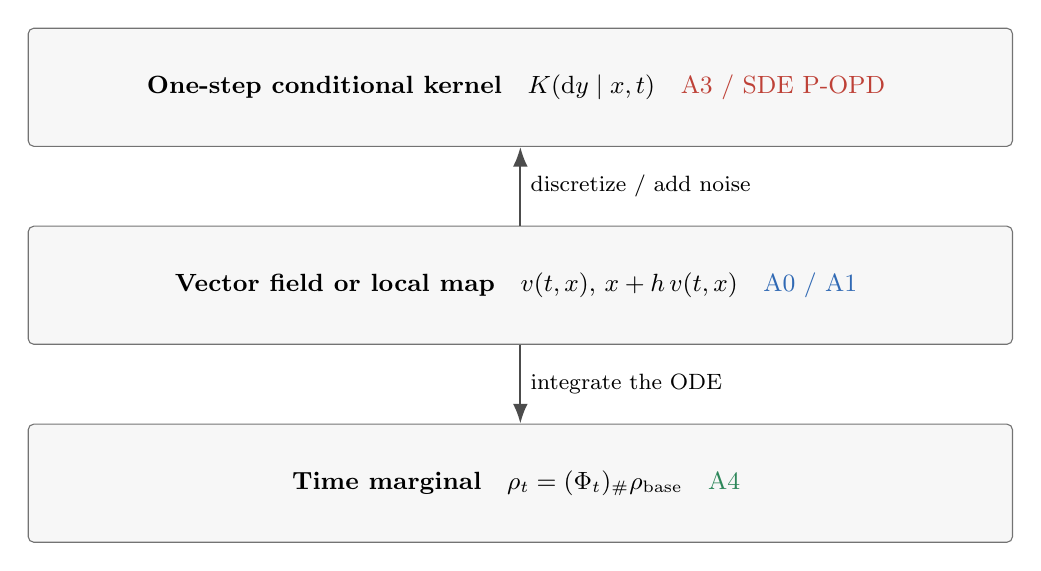
\begin{tikzpicture}[node distance=10mm]
  \node[neutralbox,minimum width=125mm,minimum height=15mm] (kernel) {
    \textbf{One-step conditional kernel}\quad
    $K(\dd y\mid x,t)$\quad
    \textcolor{teacherred}{A3 / SDE P-OPD}
  };
  \node[neutralbox,minimum width=125mm,minimum height=15mm,below=of kernel] (field) {
    \textbf{Vector field or local map}\quad
    $v(t,x)$, $x+h\,v(t,x)$\quad
    \textcolor{oldblue}{A0 / A1}
  };
  \node[neutralbox,minimum width=125mm,minimum height=15mm,below=of field] (marginal) {
    \textbf{Time marginal}\quad
    $\rho_t=(\Phi_t)_\#\rho_{\mathrm{base}}$\quad
    \textcolor{studentgreen}{A4}
  };
  \draw[flowarrow] (field.north) -- node[right,font=\footnotesize] {discretize / add noise} (kernel.south);
  \draw[flowarrow] (field.south) -- node[right,font=\footnotesize] {integrate the ODE} (marginal.north);
\end{tikzpicture}
\caption{The three layers must not be interchanged.  A3 mixes stochastic one-step kernels, A0/A1
compare deterministic field outputs, and A4 mixes the distributions of states reached at each
time.}
\label{fig:three-layers}
\end{figure}

For an ODE Euler step,
\begin{equation}
K_j(\dd y\mid x,t)=\delta_{x+h\,v_j(t,x)}(\dd y).
\end{equation}
The direct KL between two unequal Dirac kernels is infinite.  More specifically, if
\begin{equation}
Q_\alpha
=(1-\alpha)\delta_{F_{\mathrm{old}}(x)}
+\alpha\delta_{F_T(x)}
\end{equation}
and $F_{\mathrm{old}}(x)\neq F_T(x)$, then
\begin{equation}
\KL(\delta_y\Vert Q_\alpha)
=
\begin{cases}
-\log(1-\alpha), & y=F_{\mathrm{old}}(x),\\
-\log\alpha, & y=F_T(x),\\
+\infty, & \text{otherwise}.
\end{cases}
\label{eq:dirac-mixture-kl}
\end{equation}
There is no smooth transition-likelihood trust region around the old map.  This is the
obstruction that prevents the exact SDE responsibility gate from surviving the zero-noise limit.

A4 changes the probability object.  ODE \emph{marginals} can have ordinary densities even though
their conditional transitions are Dirac measures.  The target is therefore a mixture of
$\rho_{\mathrm{old},t}$ and $\rho_{T,t}$, not a mixture of their deterministic next-state atoms.

\begin{tcolorbox}[colback=blue!4,colframe=blue!50!black,title=One-sentence definition]
A4 chooses the old or teacher ODE once per generated trajectory, uses the selected trajectory
state and velocity as a CFM training pair, and fits one deterministic student field whose
time marginals equal the old/teacher marginal mixture in the population limit.
\end{tcolorbox}

\subsection{Why the P-OPD result motivates A4}

For shared-covariance Gaussian SDE kernels, P-OPD uses the exact transition posterior.  Its
detached gated quadratic matches the transition-mixture KL \emph{first derivative locally} at the
behavior student; it is not a global equality of objectives.  This is the flow-transition
analogue of the external probability mixture in TOP-D~\cite{topd} and the transition view used by
DiffusionOPD~\cite{diffusionopd}.

The complete-latent responsibility concentrates when the teacher and old transition means are
separated.
The companion analysis
\path{docs/xopd/core/p_opd/popd_exact_sum_gate_saturation.tex} measured a median responsibility of
$8\times10^{-12}$ and $75.4\%$ of transitions below $0.01$ at the exact latent-sum setting in a
9B$\to$4B probe.  Removing SDE noise does not repair this problem: it makes the transition
supports singular.

A4 keeps ODE sampling efficiency and an exact probability-mixture target, but pays for a
different resource: samples from the teacher trajectory marginal.  It therefore gives up strict
student-only on-policy sampling whenever $\alpha>0$.

%% ============================================================
\section{Flow Matching from scratch}
\label{sec:fm}
%% ============================================================

\subsection{From a vector field to a density path}

Let $\Phi_t^v(z)$ be the solution of \eqref{eq:basic-ode} that starts at $z$.  The density at
time $t$ is the pushforward
\begin{equation}
\rho_t=(\Phi_t^v)_\#\rho_{\mathrm{base}}.
\label{eq:pushforward}
\end{equation}
Probability mass is neither created nor destroyed.  Infinitesimally, this is expressed by the
continuity equation
\begin{equation}
\partial_t\rho_t(x)+\nabla_x\!\cdot\!\bigl(\rho_t(x)v_t(x)\bigr)=0.
\label{eq:continuity}
\end{equation}
The product $\rho_tv_t$ is the probability \emph{flux}: density times local velocity.

\subsection{The ordinary Flow Matching loss}

Suppose a target density path $q_t$ and one velocity field $u_t$ satisfying
\begin{equation}
\partial_tq_t+\nabla\!\cdot(q_tu_t)=0
\label{eq:target-continuity}
\end{equation}
are known.  Flow Matching trains
\begin{equation}
\mathcal L_{\mathrm{FM}}(\theta)
=
\E_{C,\;t\sim\omega,\;X_t\sim q_t(\cdot\mid C)}
\left[
  \norm{\vtheta(t,X_t,C)-u_t(X_t,C)}^2
\right].
\label{eq:fm-loss}
\end{equation}
At zero population loss, integrating $\vtheta=u$ from the same base law generates $q_t$,
provided the ODE is well posed.

The difficulty is that $u_t(x)$ is often an intractable conditional expectation.  Conditional
Flow Matching (CFM)~\cite{flowmatching} replaces it by sample-wise labels.

\begin{proposition}[The CFM regression identity]
\label{prop:generic-cfm}
Let $(X_t,V_t)$ be any joint training pair such that $X_t\sim q_t$ and
\begin{equation}
u_t(x)=\E[V_t\mid X_t=x,t].
\label{eq:conditional-velocity}
\end{equation}
Then
\begin{align}
\E\norm{\vtheta(t,X_t)-V_t}^2
&=
\E\norm{\vtheta(t,X_t)-u_t(X_t)}^2
\nonumber\\
&\quad+
\E\norm{V_t-u_t(X_t)}^2.
\label{eq:generic-cfm}
\end{align}
The final term is independent of $\theta$.  CFM and FM therefore have identical population
gradients and minimizers.
\end{proposition}

\begin{proof}
Write
\[
\vtheta-V_t=(\vtheta-u_t)+(u_t-V_t)
\]
and expand the square.  Conditioned on $(t,X_t)$, the cross term is zero because
\[
\E[u_t(X_t)-V_t\mid t,X_t]=0.
\]
The remaining two squared terms give \eqref{eq:generic-cfm}.
\end{proof}

\subsection{Event sum, event mean, and RMS}

For latent shape $(C,H,W)$ or $(N_{\mathrm{tokens}},C)$, let $D$ be the number of non-batch
elements.  Two common losses are
\begin{equation}
\ell_{\mathrm{sum}}=\sum_{i=1}^D e_i^2,
\qquad
\ell_{\mathrm{mean}}=\frac1D\sum_{i=1}^D e_i^2,
\qquad
\operatorname{RMS}(e)=\sqrt{\ell_{\mathrm{mean}}}.
\label{eq:sum-mean-rms}
\end{equation}
Multiplying the entire objective by $1/D$ does not change its population minimizer at a fixed
shape, but it changes gradient and trust-radius scales.  The implementation uses
the event mean for stable cross-resolution optimization and logs both RMS and L2 scales.

\begin{lstlisting}[style=python,caption={Equivalent target, different optimization scale.}]
error = velocity_student.float() - velocity_target.float()
event_axes = tuple(range(1, error.ndim))

loss_sum_per_sample = error.square().sum(dim=event_axes)   # joint event scale
loss_mean_per_sample = error.square().mean(dim=event_axes) # resolution-stable scale
error_rms = loss_mean_per_sample.sqrt()
\end{lstlisting}

\begin{tcolorbox}[colback=yellow!5,colframe=yellow!45!black,title=Scale rule]
Use one convention consistently in the loss, trust radius, diagnostics, and ablations.  Do not
call an event mean a joint likelihood.  A4 itself is a marginal CFM construction; its practical
mean-MSE normalization is an optimization choice, not a density-ratio approximation.
\end{tcolorbox}

%% ============================================================
\section{Constructing the A4 marginal path}
\label{sec:construction}
%% ============================================================

\subsection{Two source ODEs}

Fix $C=c$ and suppress it from the notation.  The old and teacher source paths satisfy
\begin{align}
\partial_t\rho_{\mathrm{old},t}
+\nabla\!\cdot(\rho_{\mathrm{old},t}\vold)&=0,
\nonumber\\
\partial_t\rho_{T,t}
+\nabla\!\cdot(\rho_{T,t}\vT)&=0,
\label{eq:source-continuity}\\
\rho_{\mathrm{old},0}=\rho_{T,0}
&=\rho_{\mathrm{base}}.
\nonumber
\end{align}
Choose $\alpha\in[0,1]$.  The branch variable used below is independent of $(Z,t)$ conditional on
$C$.  Define the target marginal
\begin{equation}
q_t
=(1-\alpha)\rho_{\mathrm{old},t}
+\alpha\rho_{T,t}.
\label{eq:a4-q}
\end{equation}
At every $t$, $q_t$ literally samples the old marginal with probability $1-\alpha$ and the
teacher marginal with probability $\alpha$.

\subsection{The source-mixture flux selects a velocity}

The mixture density alone is not enough; a flow also needs a flux.  The source trajectories
select the natural mixture flux
\begin{equation}
q_tu_t
=(1-\alpha)\rho_{\mathrm{old},t}\vold
+\alpha\rho_{T,t}\vT.
\label{eq:a4-flux}
\end{equation}

\begin{proposition}[The mixture path is a valid Flow Matching path]
\label{prop:mixture-continuity}
The pair $(q_t,u_t)$ satisfies
\begin{equation}
\partial_tq_t+\nabla\!\cdot(q_tu_t)=0,
\qquad
q_0=\rho_{\mathrm{base}}.
\label{eq:a4-continuity}
\end{equation}
\end{proposition}

\begin{proof}
Substitute \eqref{eq:a4-q} and \eqref{eq:a4-flux}:
\begin{align*}
\partial_tq_t+\nabla\!\cdot(q_tu_t)
&=
(1-\alpha)
\left[
  \partial_t\rho_{\mathrm{old},t}
  +\nabla\!\cdot(\rho_{\mathrm{old},t}\vold)
\right]\\
&\quad+
\alpha
\left[
  \partial_t\rho_{T,t}
  +\nabla\!\cdot(\rho_{T,t}\vT)
\right]
=0.
\end{align*}
The initial equality follows because both source ODEs start from the same base law.
\end{proof}

A density path can admit another velocity that differs from $u_t$ by a $q_t$-divergence-free
field.  Thus $u_t$ is not the only imaginable field for $q_t$; it is the specific source-mixture
velocity learned by the two-source CFM joint distribution.

\subsection{Marginal responsibility}

Where $q_t(x)>0$, define
\begin{equation}
\gamma_t(x)
=
\frac{\alpha\rho_{T,t}(x)}{
  (1-\alpha)\rho_{\mathrm{old},t}(x)+\alpha\rho_{T,t}(x)
}.
\label{eq:a4-gamma}
\end{equation}
Dividing \eqref{eq:a4-flux} by $q_t$ gives
\begin{equation}
\boxed{
u_t(x)
=(1-\gamma_t(x))\vold(t,x)
+\gamma_t(x)\vT(t,x)
}.
\label{eq:a4-u}
\end{equation}

The coefficient is state dependent:
\begin{itemize}[leftmargin=1.5em]
\item where the old marginal dominates, $\gamma_t(x)\approx0$ and $u_t\approx\vold$;
\item where the teacher marginal dominates, $\gamma_t(x)\approx1$ and $u_t\approx\vT$;
\item where both marginals overlap, the velocity interpolates according to posterior branch
      probability.
\end{itemize}
This is why the constant arithmetic average
$(1-\alpha)\vold+\alpha\vT$ is generally wrong.
Figure~\ref{fig:a4-branch} shows the joint sampling process that selects this particular flux.

\begin{figure}[htbp]
\centering
\resizebox{\textwidth}{!}{
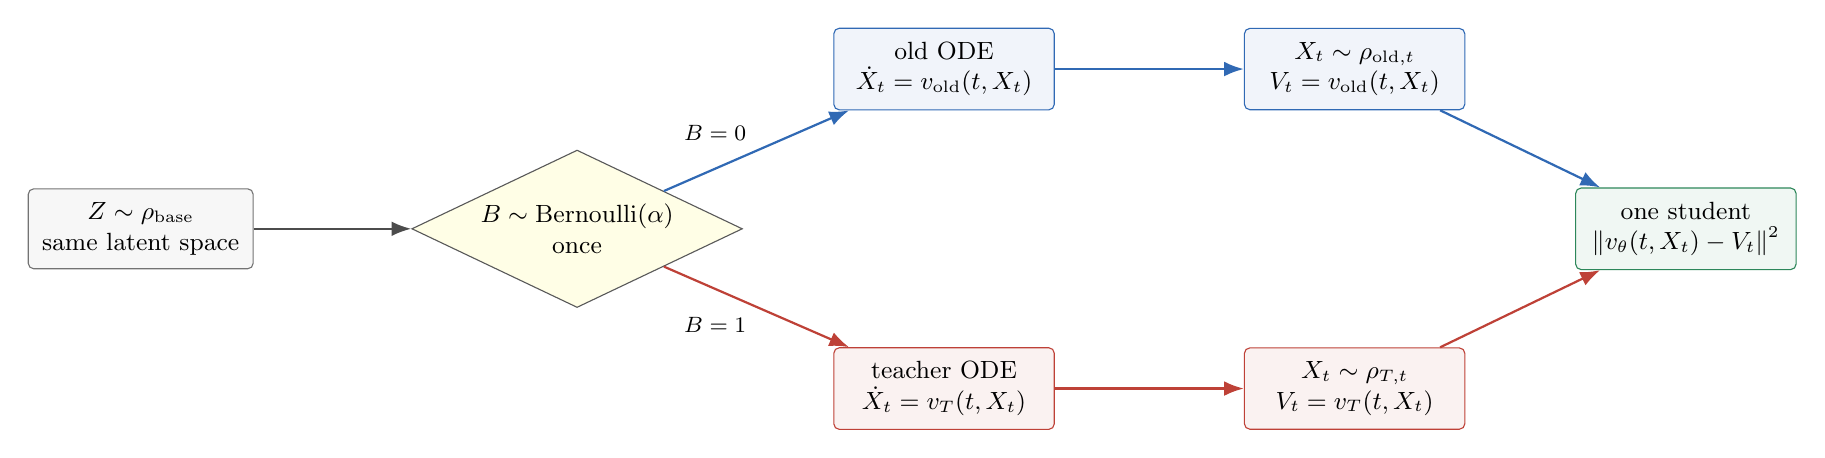
\begin{tikzpicture}[node distance=15mm and 20mm]
  \node[neutralbox] (base) {$Z\sim\rho_{\mathrm{base}}$\\same latent space};
  \node[decision,right=of base] (branch) {$B\sim\mathrm{Bernoulli}(\alpha)$\\once};
  \node[oldbox,above right=10mm and 22mm of branch] (oldflow) {
    old ODE\\$\dot X_t=\vold(t,X_t)$
  };
  \node[teacherbox,below right=10mm and 22mm of branch] (teacherflow) {
    teacher ODE\\$\dot X_t=\vT(t,X_t)$
  };
  \node[oldbox,right=24mm of oldflow] (oldpair) {
    $X_t\sim\rho_{\mathrm{old},t}$\\$V_t=\vold(t,X_t)$
  };
  \node[teacherbox,right=24mm of teacherflow] (teacherpair) {
    $X_t\sim\rho_{T,t}$\\$V_t=\vT(t,X_t)$
  };
  \node[studentbox,right=28mm of $(oldpair)!0.5!(teacherpair)$] (loss) {
    one student\\$\norm{\vtheta(t,X_t)-V_t}^2$
  };

  \draw[flowarrow] (base) -- (branch);
  \draw[flowarrow,draw=oldblue] (branch) -- node[above left,font=\footnotesize] {$B=0$} (oldflow);
  \draw[flowarrow,draw=teacherred] (branch) -- node[below left,font=\footnotesize] {$B=1$} (teacherflow);
  \draw[flowarrow,draw=oldblue] (oldflow) -- (oldpair);
  \draw[flowarrow,draw=teacherred] (teacherflow) -- (teacherpair);
  \draw[flowarrow,draw=oldblue] (oldpair) -- (loss);
  \draw[flowarrow,draw=teacherred] (teacherpair) -- (loss);
\end{tikzpicture}
}
\caption{A4 samples the branch once for the entire trajectory.  The branch determines both the
state distribution and the velocity label.  Only the student on the right receives gradients.}
\label{fig:a4-branch}
\end{figure}

\subsection{One-dimensional intuition}

Figure~\ref{fig:one-dimensional} shows a schematic equal-variance example.  The prior branch
weight is $\alpha=0.4$.  At points near the old mode the posterior teacher responsibility is
small; near the teacher mode it is large.  At a point where the two source densities are equal,
$\gamma_t(x)=\alpha$.

\begin{figure}[htbp]
\centering
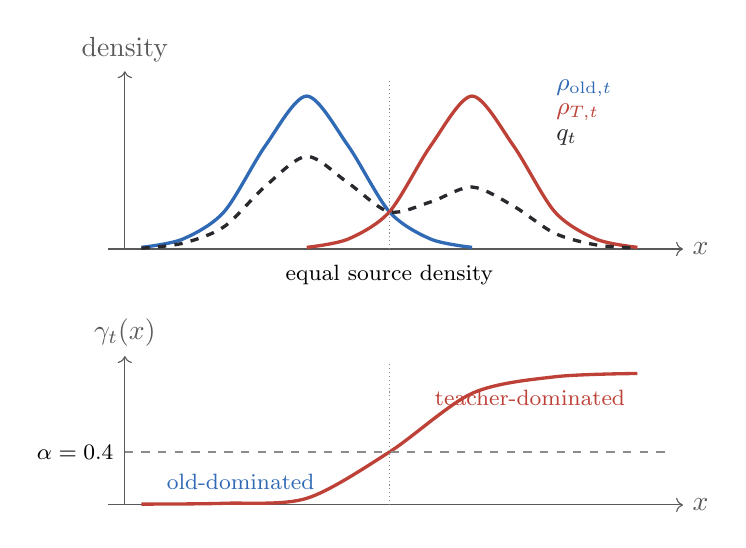
\begin{tikzpicture}[x=1.05cm,y=1.05cm]
  % Density panel
  \draw[->,black!65] (-3.4,0) -- (3.55,0) node[right] {$x$};
  \draw[->,black!65] (-3.2,0) -- (-3.2,2.15) node[above] {density};
  \draw[oldline,smooth] plot coordinates {
    (-3.0,0.02) (-2.5,0.12) (-2.0,0.45) (-1.5,1.25)
    (-1.0,1.85) (-0.5,1.25) (0.0,0.45) (0.5,0.12) (1.0,0.02)
  };
  \draw[teacherline,smooth] plot coordinates {
    (-1.0,0.02) (-0.5,0.12) (0.0,0.45) (0.5,1.25)
    (1.0,1.85) (1.5,1.25) (2.0,0.45) (2.5,0.12) (3.0,0.02)
  };
  \draw[mixline,smooth] plot coordinates {
    (-3.0,0.01) (-2.5,0.07) (-2.0,0.27) (-1.5,0.76)
    (-1.0,1.12) (-0.5,0.80) (0.0,0.45) (0.5,0.57)
    (1.0,0.75) (1.5,0.52) (2.0,0.19) (2.5,0.05) (3.0,0.01)
  };
  \node[anchor=west,text=oldblue,font=\small] at (1.9,1.95) {$\rho_{\mathrm{old},t}$};
  \node[anchor=west,text=teacherred,font=\small] at (1.9,1.65) {$\rho_{T,t}$};
  \node[anchor=west,text=mixtureblack,font=\small] at (1.9,1.35) {$q_t$};
  \draw[densely dotted,black!45] (0,0) -- (0,2.05);
  \node[font=\footnotesize,anchor=north] at (0,-0.08) {equal source density};

  % Responsibility panel
  \begin{scope}[yshift=-3.25cm]
    \draw[->,black!65] (-3.4,0) -- (3.55,0) node[right] {$x$};
    \draw[->,black!65] (-3.2,0) -- (-3.2,1.8) node[above] {$\gamma_t(x)$};
    \draw[teacherline,smooth] plot coordinates {
      (-3.0,0.01) (-2.0,0.02) (-1.0,0.08) (0.0,0.64)
      (1.0,1.35) (2.0,1.55) (3.0,1.59)
    };
    \draw[densely dotted,black!45] (0,0) -- (0,1.72);
    \draw[dashed,black!45] (-3.2,0.64) -- (3.35,0.64);
    \node[font=\footnotesize,anchor=east] at (-3.22,0.64) {$\alpha=0.4$};
    \node[font=\footnotesize,text=oldblue] at (-1.8,0.28) {old-dominated};
    \node[font=\footnotesize,text=teacherred] at (1.7,1.30) {teacher-dominated};
  \end{scope}
\end{tikzpicture}
\caption{Schematic source densities, their marginal mixture, and the posterior teacher
responsibility.  The curves are illustrative rather than measured model densities.}
\label{fig:one-dimensional}
\end{figure}

%% ============================================================
\section{Why two-source CFM needs no density ratio}
\label{sec:cfm}
%% ============================================================

\subsection{The training joint distribution}

The direct formula \eqref{eq:a4-u} appears impractical because modern flow-model densities are not
available.  The CFM identity solves this by sampling the latent branch variable explicitly:
\begin{equation}
B\sim\operatorname{Bernoulli}(\alpha),
\qquad
X_t=\Phi_t^B(Z),
\qquad
V_t=
\begin{cases}
\vold(t,X_t), & B=0,\\
\vT(t,X_t), & B=1.
\end{cases}
\label{eq:branch-pair}
\end{equation}
Marginalizing $B$ gives $X_t\sim q_t$.  Bayes' rule gives
\begin{equation}
\Pr(B=1\mid X_t=x,t)
=
\frac{\alpha\rho_{T,t}(x)}{q_t(x)}
=\gamma_t(x).
\label{eq:branch-posterior}
\end{equation}
Therefore
\begin{equation}
\E[V_t\mid X_t=x,t]
=(1-\gamma_t(x))\vold(t,x)+\gamma_t(x)\vT(t,x)
=u_t(x).
\label{eq:branch-conditional-mean}
\end{equation}

\begin{proposition}[The exact A4 CFM identity]
\label{prop:a4-cfm}
Define
\begin{equation}
\mathcal L_{\mathrm{A4}}(\theta)
=
\E_{C,\;t,\;B,\;Z}
\norm{\vtheta(t,X_t,C)-V_t}^2.
\label{eq:a4-loss}
\end{equation}
Then
\begin{align}
\mathcal L_{\mathrm{A4}}(\theta)
&=
\E_{C,\;t,\;X_t\sim q_t}
\norm{\vtheta(t,X_t,C)-u_t(X_t,C)}^2
\nonumber\\
&\quad+
\mathcal C_{\mathrm{var}},
\label{eq:a4-loss-decomposition}\\
\mathcal C_{\mathrm{var}}
&=
\E_{C,\;t,\;X_t\sim q_t}
\left[
  \gamma_t(X_t)(1-\gamma_t(X_t))
  \norm{\vT(t,X_t)-\vold(t,X_t)}^2
\right].
\label{eq:a4-label-variance}
\end{align}
The variance term is independent of $\theta$, so A4 CFM and marginal FM have identical
population gradients and minimizers.
\end{proposition}

\begin{proof}
Proposition~\ref{prop:generic-cfm} applies because
\eqref{eq:branch-conditional-mean} identifies $u_t$ as the conditional mean label.  For a
two-point random label, the conditional variance is
\[
\gamma_t(1-\gamma_t)\norm{\vT-\vold}^2,
\]
which gives \eqref{eq:a4-label-variance}.
\end{proof}

\subsection{The central implementation insight}

The density responsibility appears in the \emph{analytic population minimizer}, but not in the
Monte Carlo training recipe:
\begin{enumerate}[leftmargin=1.6em]
\item sample $B$;
\item generate a state from the corresponding ODE;
\item use that ODE's velocity as the detached label;
\item regress the current student onto the label.
\end{enumerate}
Ordinary square-loss regression learns the conditional average automatically.

\begin{lstlisting}[style=goodpython,caption={Minimal conceptual A4 training step.}]
# Conceptual code, independent of Flow-Factory plumbing.
branch = torch.rand(batch_size, device=device) < alpha

# The branch is fixed for the complete trajectory.
x_t, velocity_target = rollout_selected_source(
    branch=branch,
    initial_noise=initial_noise,
    condition=condition,
    training_time=training_time,
)
velocity_target = velocity_target.detach()

velocity_student = student.predict_velocity(
    t=training_time,
    latents=x_t,
    condition=condition,
)
event_axes = tuple(range(1, velocity_student.ndim))
loss_per_sample = (
    velocity_student.float() - velocity_target.float()
).square().mean(dim=event_axes)
loss = loss_per_sample.mean()
\end{lstlisting}

\begin{tcolorbox}[colback=green!5,colframe=green!50!black,title=No classifier and no fake-score network]
A4 does not require a classifier for $\rho_T/\rho_{\mathrm{old}}$, a CNF log-density evaluator,
or a DMD-style online fake score.  It requires the ability to \emph{sample both source
trajectories}.  The hidden branch label supplies the posterior responsibility implicitly through
conditional regression.
\end{tcolorbox}

\subsection{What the variance term means}

$\mathcal C_{\mathrm{var}}$ is irreducible label ambiguity.  At a state where both branches have
non-negligible density but prescribe different velocities, the learner observes two possible
labels.  The square-loss optimum is their posterior average $u_t(x)$.

This is not an optimization bug.  It is exactly the velocity needed to transport the mixture
marginal.  It can nevertheless be difficult for a finite network when the responsibility changes
sharply across state space.

%% ============================================================
\section{What ``exact'' means, and where it stops}
\label{sec:exactness}
%% ============================================================

\subsection{Exact population realization}

Assume:
\begin{enumerate}[leftmargin=1.6em]
\item both source densities and fluxes are sufficiently smooth;
\item $q_t(x)>0$ on the relevant region;
\item $u_t$ is continuous in $t$, Lipschitz in $x$, and has at most linear growth;
\item the model can represent $u_t$ and population optimization reaches it;
\item the fitted representative is regular enough to define a unique ODE.
\end{enumerate}
Then
\begin{equation}
\dot X_t=u_t(X_t),
\qquad
X_0\sim\rho_{\mathrm{base}}
\label{eq:mixture-ode}
\end{equation}
has marginals
\begin{equation}
(\Phi_t^u)_\#\rho_{\mathrm{base}}
=q_t
=(1-\alpha)\rho_{\mathrm{old},t}+\alpha\rho_{T,t}.
\label{eq:exact-mixture}
\end{equation}
This is exactness at the \emph{time-marginal} level.  The deterministic $u$-trajectory law is not
the same as the random path law that chooses old or teacher once; only their one-time marginals
agree.

\subsection{The proximal contraction}

Assume $\rho_{\mathrm{old},t}$ is absolutely continuous with respect to $\rho_{T,t}$ and the
displayed KL is finite.  For the Wasserstein statement, let $p\ge1$ and assume both laws have
finite $p$-th moments.  Then, at every time,
\begin{align}
\norm{q_t-\rho_{T,t}}_1
&=
(1-\alpha)
\norm{\rho_{\mathrm{old},t}-\rho_{T,t}}_1,
\label{eq:l1-contraction}\\
\KL(q_t\Vert\rho_{T,t})
&\le
(1-\alpha)\KL(\rho_{\mathrm{old},t}\Vert\rho_{T,t}),
\label{eq:kl-contraction}\\
W_p^p(q_t,\rho_{T,t})
&\le
(1-\alpha)W_p^p(\rho_{\mathrm{old},t},\rho_{T,t}).
\label{eq:wasserstein-contraction}
\end{align}
The first identity follows by factoring the signed density difference.  The KL inequality follows
from convexity in its first argument.  The Wasserstein bound follows by coupling an
$\alpha$ fraction of teacher mass to itself and transporting only the remaining old mass.

If every outer iteration fits the mixture path exactly and refreshes
$\rho_{\mathrm{old},t}\leftarrow\rho_{\theta,t}$, then
\begin{equation}
\norm{\rho_{k+1,t}-\rho_{T,t}}_1
=(1-\alpha)
\norm{\rho_{k,t}-\rho_{T,t}}_1.
\label{eq:iterative-contraction}
\end{equation}
This is the clean deterministic mixture-contraction story.  A real LoRA update introduces
projection and optimization error.

\subsection{Finite capacity}

Let $\widehat v$ be the trained field and
\begin{equation}
e_t(x)=\widehat v(t,x)-u_t(x).
\end{equation}
If both laws have finite second moments, the fitting error below is integrable,
$\widehat v$ is $L$-Lipschitz, and the exact and approximate ODEs start from the same noise, then
a Gr\"onwall coupling gives
\begin{equation}
W_2^2(\widehat\rho_t,q_t)
\le
t\int_0^t
e^{2L(t-s)}
\E_{X_s\sim q_s}\norm{e_s(X_s)}^2\dd s.
\label{eq:capacity-bound}
\end{equation}
Consequently,
\begin{equation}
W_2(\widehat\rho_t,\rho_{T,t})
\le
W_2(\widehat\rho_t,q_t)
+
(1-\alpha)^{1/2}
W_2(\rho_{\mathrm{old},t},\rho_{T,t})
\label{eq:practical-bound}
\end{equation}
for $p=2$.  The first term is the price of finite fitting; the second is the ideal proximal
contraction.

\subsection{Low overlap and stiffness}

Where both source densities are positive,
\begin{equation}
\nabla\gamma_t
=
\gamma_t(1-\gamma_t)
\left(
  \nabla\log\rho_{T,t}
  -\nabla\log\rho_{\mathrm{old},t}
\right).
\label{eq:gamma-gradient}
\end{equation}
Low-overlap marginals can create a thin boundary where $\gamma_t$ switches rapidly and $u_t$
changes from $\vold$ to $\vT$.  The training labels remain valid, but a small student or a coarse
ODE solver can smooth or misintegrate that boundary.

\begin{tcolorbox}[colback=red!4,colframe=red!45!black,title=Do not transfer ideal guarantees to a finite run]
Equations~\eqref{eq:l1-contraction}--\eqref{eq:wasserstein-contraction} describe the target
mixture $q_t$.  They do not prove that a finite LoRA student, finite batch, sparse timestep
subsample, or imperfect optimizer achieves the same contraction.  The measured CFM fitting error
and rollout drift must be logged separately.
\end{tcolorbox}

%% ============================================================
\section{Should the teacher weight change during training?}
\label{sec:dynamic-alpha}
%% ============================================================

\subsection{First separate outer-loop time from ODE time}

There are two different proposals that are both easily called ``dynamic alpha'':
\begin{enumerate}[leftmargin=1.6em]
\item an \emph{outer-loop schedule} $\alpha_k$, held fixed over the complete ODE path and all
      timesteps of training iteration $k$;
\item an \emph{ODE-time schedule} $\alpha(t)$ that changes between noise and data within one
      trajectory.
\end{enumerate}
Only the first is an immediate extension of implemented A4.  At outer iteration $k$, define
\begin{equation}
q_{k,t}
:=
(1-\alpha_k)\rho_{k,t}
+\alpha_k\rho_{T,t},
\qquad
B_k\sim\operatorname{Bernoulli}(\alpha_k),
\label{eq:scheduled-outer-mixture}
\end{equation}
where one $B_k$ is still fixed for a complete sampled trajectory.  Conditional on $k$,
Propositions~\ref{prop:mixture-continuity} and~\ref{prop:a4-cfm} apply without modification.

The same is \emph{not} true for a prior that changes with ODE time.  If
\[
q_t=(1-\alpha(t))\rho_{\mathrm{old},t}+\alpha(t)\rho_{T,t}
\]
and one uses the old source-mixture flux from \eqref{eq:a4-flux}, direct differentiation gives
\begin{equation}
\partial_tq_t+
\nabla\!\cdot\left[
  (1-\alpha(t))\rho_{\mathrm{old},t}\vold
  +\alpha(t)\rho_{T,t}\vT
\right]
=
\alpha'(t)\left(\rho_{T,t}-\rho_{\mathrm{old},t}\right),
\label{eq:time-alpha-continuity-defect}
\end{equation}
which is generally nonzero.  A valid deterministic flow would need an additional transfer flux
$J_t$ satisfying
\begin{equation}
\nabla\!\cdot J_t
=-\alpha'(t)\left(\rho_{T,t}-\rho_{\mathrm{old},t}\right).
\label{eq:time-alpha-transfer-flux}
\end{equation}
Equivalently, a stochastic construction would need a coherent branch-switching process rather
than independent Bernoulli labels at different timesteps.  Neither correction is supplied by
one-branch A4 CFM.

\begin{tcolorbox}[colback=yellow!6,colframe=yellow!55!black,title=Safe meaning of a dynamic teacher weight]
In the current algorithm, schedule $\alpha$ by \emph{outer optimizer epoch or outer policy
refresh}, then keep that value fixed across ODE time $t$ and across every callback of a sampled
trajectory.  Do not silently turn it into $\alpha(t)$ inside the denoising solver.
\end{tcolorbox}

\subsection{Exact contraction under an outer-loop schedule}

Let
\begin{equation}
D_k(t):=\norm{\rho_{k,t}-\rho_{T,t}}_1.
\end{equation}
Under exact population fitting of \eqref{eq:scheduled-outer-mixture},
\begin{equation}
D_{k+1}(t)
=(1-\alpha_k)D_k(t),
\qquad
D_K(t)
=
\left[\prod_{j=0}^{K-1}(1-\alpha_j)\right]D_0(t).
\label{eq:scheduled-contraction}
\end{equation}
Thus the effective teacher mass accumulated by iteration $K$ is
\begin{equation}
A_{\mathrm{eff}}(K)
:=
1-\prod_{j=0}^{K-1}(1-\alpha_j).
\label{eq:effective-teacher-mass}
\end{equation}
This quantity, not the final value $\alpha_{K-1}$ alone, controls ideal progress.

If every $\alpha_k<1$, convergence to the teacher requires
\begin{equation}
\prod_{k=0}^{\infty}(1-\alpha_k)=0,
\quad\text{equivalently}\quad
\sum_{k=0}^{\infty}-\log(1-\alpha_k)=\infty.
\label{eq:schedule-convergence-condition}
\end{equation}
When the schedule is bounded away from one, the familiar sufficient and essentially equivalent
condition is $\sum_k\alpha_k=\infty$.  Important examples are:
\begin{itemize}[leftmargin=1.5em]
\item constant $\alpha_k=\alpha>0$: geometric contraction;
\item harmonic decay $\alpha_k=c/(k+b)$: polynomial contraction and eventual convergence;
\item exponential decay $\alpha_k=\alpha_0r^k$, $0<r<1$: finite total teacher mass, so the ideal
      student generally stops short of the teacher;
\item decay to a positive floor $\alpha_{\min}>0$: eventual geometric contraction.
\end{itemize}

In the exact model, schedules with the same multiset of $\alpha_k$ values have the same final
product in \eqref{eq:scheduled-contraction}; front-loading or back-loading those values only
changes the intermediate path.  Their practical behavior differs because optimization error,
network capacity, and branch-sampling noise depend on the current student--teacher gap.

\subsection{What alpha does to the optimization problem}

For a fixed outer iteration, write the branch-conditioned stochastic gradients as $G_{\mathrm O}$
and $G_{\mathrm T}$.  The A4 gradient has mean
\begin{equation}
\E[G]
=(1-\alpha)\E[G_{\mathrm O}]
+\alpha\E[G_{\mathrm T}],
\label{eq:alpha-gradient-mean}
\end{equation}
and the law of total variance contains the between-branch term
\begin{equation}
\operatorname{Var}(G)
=
(1-\alpha)\operatorname{Var}(G_{\mathrm O})
+\alpha\operatorname{Var}(G_{\mathrm T})
+\alpha(1-\alpha)
\norm{\E[G_{\mathrm T}]-\E[G_{\mathrm O}]}^2.
\label{eq:alpha-gradient-variance}
\end{equation}
At the beginning of an outer iteration the current student equals, or is close to, the frozen old
student.  The old-branch gradient is then small and the teacher branch supplies most of the
learning signal.  In the simplified limit $G_{\mathrm O}=0$ and deterministic $G_{\mathrm T}=g$,
the signal magnitude is $\alpha\norm{g}$ while the branch standard deviation is
$\sqrt{\alpha(1-\alpha)}\norm{g}$.  The single-sample signal-to-noise ratio is therefore
\begin{equation}
\sqrt{\frac{\alpha}{1-\alpha}}.
\label{eq:bernoulli-gradient-snr}
\end{equation}
Reducing $\alpha$ reduces the expected update, but it does \emph{not} automatically make that
update statistically smoother: it also makes teacher trajectories rarer.  With $N$ independent
rows, only $N\alpha$ teacher rows are expected.  Very small $\alpha$ can produce empty teacher
subsets, weak signal, and high run-to-run variation.  In the current rank-synchronous FSDP path,
all ranks intentionally reuse the same branch pattern to preserve collective call order, so the
effective number of independent routing rows is the local pattern size rather than a
world-size-multiplied batch.  This makes small-alpha sampling noise especially relevant.

The ideal distributional movement in one refresh is
\begin{equation}
\norm{q_{k,t}-\rho_{k,t}}_1
=\alpha_k D_k(t).
\label{eq:ideal-trust-step}
\end{equation}
This equation gives a precise interpretation of ``learning pressure'': it depends on both
$\alpha_k$ and the remaining student--teacher discrepancy.  Increasing $\alpha_k$ can still keep
the actual movement constant or decreasing if $D_k$ falls sufficiently fast.

\subsection{Finite fitting error changes the answer}

Let $\varepsilon_k(\alpha_k)$ summarize the discrepancy introduced by finite LoRA capacity,
finite samples, timestep subsampling, and incomplete optimization.  A generic practical
recursion is
\begin{equation}
D_{k+1}
\le
(1-\alpha_k)D_k+\varepsilon_k(\alpha_k).
\label{eq:inexact-scheduled-recursion}
\end{equation}
Unrolling it yields
\begin{equation}
D_K
\le
\left[\prod_{j=0}^{K-1}(1-\alpha_j)\right]D_0
+
\sum_{j=0}^{K-1}
\varepsilon_j(\alpha_j)
\prod_{\ell=j+1}^{K-1}(1-\alpha_\ell).
\label{eq:inexact-scheduled-bound}
\end{equation}
This exposes the real tradeoff:
\begin{itemize}[leftmargin=1.5em]
\item larger $\alpha_k$ gives stronger ideal contraction;
\item a large teacher jump can increase $\varepsilon_k(\alpha_k)$ when the target field is hard
      for the student or optimizer;
\item substantial teacher weight at later iterations attenuates errors accumulated earlier;
\item annealing $\alpha_k$ toward zero preserves the old field, but also weakens correction of
      both teacher discrepancy and earlier fitting error.
\end{itemize}
If fitting error were independent of alpha, larger alpha would always improve this bound.
Annealing is justified only by evidence that the fitting or stability error grows enough with
teacher pressure to dominate the stronger contraction.

\subsection{Increasing teacher weight: a continuation interpretation}

An increasing schedule is a valid homotopy or trust-region strategy:
\begin{equation}
0<\alpha_0\le\alpha_1\le\cdots\le\alpha_{\max}.
\end{equation}
Early mixtures remain close to the old student, so a limited-capacity LoRA adapter does not need
to represent the full teacher displacement at once.  As the gap $D_k$ shrinks, alpha can grow
while the actual step $\alpha_kD_k$ in \eqref{eq:ideal-trust-step} remains controlled.  This
formalizes the useful part of the ``start with little teacher, then approach teacher'' intuition.

The wording requires care: increasing alpha does not itself reduce teacher pressure; it increases
the nominal teacher probability.  Pressure can nevertheless fall because the teacher and old
fields have become closer.  A practical trust-region rule would estimate a gap statistic $M_k$,
for example an exponential moving average of
\texttt{student\_target\_gap\_rms} on teacher branches, and set
\begin{equation}
\alpha_{k+1}
=
\operatorname{clip}\left(
  \frac{\delta}{M_k+\epsilon},
  \alpha_{\min},
  \alpha_{\max}
\right),
\label{eq:gap-adaptive-alpha}
\end{equation}
where $\delta$ is a desired update-pressure budget.  As $M_k$ decreases, the controller naturally
raises teacher exposure.

Potential disadvantages are slower early progress, too few teacher samples, and an abrupt late
increase if the schedule is based only on iteration count.  A floor on expected teacher rows and
slow, epoch-level updates with hysteresis are safer than per-batch reactions.

\subsection{Decreasing teacher weight: stabilization with a bias cost}

A decreasing schedule can make late updates more proximal to the current student:
\begin{equation}
\alpha_0\ge\alpha_1\ge\cdots\ge\alpha_{\min}.
\end{equation}
It can be useful when teacher-branch loss, gradient clipping, rollout failures, or fitting error
increase late in training.  More old trajectories then act as a self-consistency anchor.

However, decreasing alpha is not analogous to an ordinary learning-rate decay.  It changes the
\emph{target distribution}.  If alpha decays too quickly to zero, condition
\eqref{eq:schedule-convergence-condition} fails and even an ideal learner retains a nonzero
teacher discrepancy.  This is exactly the wrong default if training is already stable: reducing
teacher weight weakens the only force that moves the refreshed old student toward the teacher.

Safer variants are:
\begin{itemize}[leftmargin=1.5em]
\item decay only after a measured instability event, with recovery when diagnostics normalize;
\item decay to a positive floor rather than zero;
\item use a harmonic tail if asymptotic teacher convergence is desired;
\item decay the optimizer learning rate while keeping alpha fixed when the problem is ordinary
      parameter-update noise rather than a bad target mixture.
\end{itemize}

\subsection{Recommendation and ablation design}

\begin{tcolorbox}[colback=green!5,colframe=green!50!black,title=Recommended default]
A dynamic schedule is \emph{not theoretically necessary}.  Start with the static
$\alpha=0.5$ baseline because it has geometric ideal contraction, balanced branch coverage, and
the simplest interpretation.  Add scheduling only after branch-conditioned loss, target-gap,
gradient-norm, clipping, and evaluation curves identify either an excessive initial jump or a
late stability problem.
\end{tcolorbox}

For a controlled study, compare:
\begin{enumerate}[leftmargin=1.6em]
\item static $\alpha=0.5$;
\item increasing continuation, for example $0.1\rightarrow0.5$;
\item decreasing stabilization with a floor, for example $0.5\rightarrow0.1$ rather than zero;
\item a gap-adaptive trust-region schedule such as \eqref{eq:gap-adaptive-alpha}.
\end{enumerate}
Report both the schedule and $A_{\mathrm{eff}}(K)$ from
\eqref{eq:effective-teacher-mass}.  Matching only the number of epochs is not a fair comparison:
different schedules change ideal contraction, the number of teacher trajectories, and expected
rollout cost.  At minimum, log the realized teacher branch count, teacher/old conditioned losses,
teacher-branch target gap, gradient norm and clipping rate, and fixed student-only evaluation.

%% ============================================================
\section{Methods that look like A4 but are not A4}
\label{sec:not-a4}
%% ============================================================

\subsection{A compact comparison}

\begin{center}
\begin{tabular}{@{}
  >{\raggedright\arraybackslash}p{0.10\textwidth}
  >{\raggedright\arraybackslash}p{0.24\textwidth}
  >{\raggedright\arraybackslash}p{0.28\textwidth}
  >{\raggedright\arraybackslash}p{0.27\textwidth}
@{}}
\toprule
method & sampled states & target & mathematical object\\
\midrule
A0 direct OPD
& $X_t\sim\rho_{\mathrm{old},t}$
& $\vT(t,X_t)$
& old-occupancy field regression\\
\addlinespace
A1 field barycenter
& $X_t\sim\rho_{\mathrm{old},t}$
& $(1-\alpha)\vold+\alpha\vT$
& quadratic field geometry\\
\addlinespace
A3 P-OPD
& old SDE transition $(X_t,Y)$
& Gaussian transition responsibility
& one-step stochastic-kernel mixture\\
\addlinespace
\textbf{A4}
& $X_t\sim(1-\alpha)\rho_{\mathrm{old},t}+\alpha\rho_{T,t}$
& velocity of the sampled source branch
& ODE time-marginal mixture\\
\bottomrule
\end{tabular}
\end{center}

\subsection{Wrong variant 1: teacher on old states}

\begin{lstlisting}[style=badpython,caption={This is A0, not A4.}]
# WRONG if the intended method is A4.
x_t = old_trajectory.state_at(t)
velocity_target = teacher.predict_velocity(t=t, latents=x_t)
loss = mse(student.predict_velocity(t=t, latents=x_t), velocity_target)
\end{lstlisting}

The teacher target is valid, but every query state still follows $\rho_{\mathrm{old},t}$.
No sample ever comes from $\rho_{T,t}$, so the training state marginal is not $q_t$.

\begin{lstlisting}[style=goodpython,caption={The source branch controls both state and target.}]
branch = sample_once_for_the_trajectory(alpha)
if branch == OLD:
    x_t = old_trajectory.state_at(t)
    velocity_target = old_trajectory.velocity_at(t)
else:
    x_t = teacher_trajectory.state_at(t)
    velocity_target = teacher_trajectory.velocity_at(t)
\end{lstlisting}

\subsection{Wrong variant 2: re-sample the branch every Euler step}

If independent branch labels $B_\ell$ are drawn at every step,
\begin{equation}
X_{\ell+1}
=X_\ell+h_\ell v_{B_\ell}(t_\ell,X_\ell),
\qquad
B_\ell\overset{\mathrm{iid}}{\sim}\operatorname{Bernoulli}(\alpha),
\label{eq:fast-switch}
\end{equation}
then the conditional mean field is
\begin{equation}
\bar v=(1-\alpha)\vold+\alpha\vT.
\label{eq:arithmetic-field}
\end{equation}
The switching variance vanishes with the step size, so the continuous-time limit is the
arithmetic-average ODE, not the A4 marginal-mixture ODE.  Their gap is
\begin{equation}
\bar v-u_t
=(\alpha-\gamma_t)(\vT-\vold).
\label{eq:average-gap}
\end{equation}
Figure~\ref{fig:branch-trap} contrasts the two branch lifetimes.

\begin{figure}[htbp]
\centering
\resizebox{\textwidth}{!}{
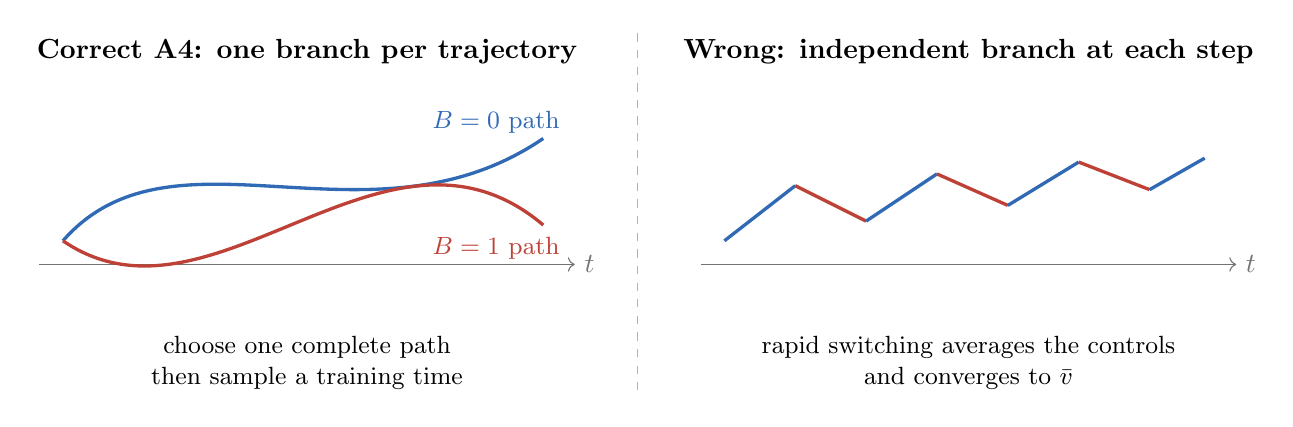
\begin{tikzpicture}[x=1cm,y=1cm]
  % Correct panel
  \node[font=\bfseries] at (0,2.7) {Correct A4: one branch per trajectory};
  \draw[->,black!55] (-3.4,0) -- (3.4,0) node[right] {$t$};
  \coordinate (startL) at (-3.1,0.3);
  \draw[oldline] (-3.1,0.3) .. controls (-1.7,1.9) and (0.8,0.1) .. (3.0,1.6);
  \draw[teacherline] (-3.1,0.3) .. controls (-1.2,-1.0) and (1.0,2.2) .. (3.0,0.5);
  \node[text=oldblue,font=\small] at (2.4,1.8) {$B=0$ path};
  \node[text=teacherred,font=\small] at (2.4,0.2) {$B=1$ path};
  \node[font=\small,align=center] at (0,-1.25) {choose one complete path\\then sample a training time};

  % Divider
  \draw[dashed,black!30] (4.2,-1.6) -- (4.2,3.0);

  % Wrong panel
  \begin{scope}[xshift=8.4cm]
    \node[font=\bfseries] at (0,2.7) {Wrong: independent branch at each step};
    \draw[->,black!55] (-3.4,0) -- (3.4,0) node[right] {$t$};
    \draw[oldline] (-3.1,0.3) -- (-2.2,1.0);
    \draw[teacherline] (-2.2,1.0) -- (-1.3,0.55);
    \draw[oldline] (-1.3,0.55) -- (-0.4,1.15);
    \draw[teacherline] (-0.4,1.15) -- (0.5,0.75);
    \draw[oldline] (0.5,0.75) -- (1.4,1.30);
    \draw[teacherline] (1.4,1.30) -- (2.3,0.95);
    \draw[oldline] (2.3,0.95) -- (3.0,1.35);
    \node[font=\small,align=center] at (0,-1.25) {rapid switching averages the controls\\and converges to $\bar v$};
  \end{scope}
\end{tikzpicture}
}
\caption{A path-law mixture chooses one source trajectory.  Independent per-step switches solve a
different problem and converge to the A1-style arithmetic field.}
\label{fig:branch-trap}
\end{figure}

\begin{lstlisting}[style=badpython,caption={Per-step branch sampling changes the target method.}]
# WRONG: this converges to the arithmetic-average field.
for timestep_index in range(num_steps):
    branch = torch.rand(batch_size) < alpha  # re-drawn every step
    velocity = torch.where(branch, velocity_teacher, velocity_old)
    latents = latents + dt[timestep_index] * velocity
\end{lstlisting}

\subsection{A3/P-OPD is a different probability mixture}

A3 uses a sampled SDE next state $Y$ and computes
\begin{equation}
\gamma_T(Y)
=
\frac{\alpha p_T(Y\mid X_t)}
{(1-\alpha)p_{\mathrm{old}}(Y\mid X_t)+\alpha p_T(Y\mid X_t)}.
\label{eq:a3-gate}
\end{equation}
This is an exact \emph{transition} posterior under shared positive covariance.  A4 instead uses
the posterior branch probability of a \emph{time marginal}, but never evaluates it.  Reusing the
current P-OPD responsibility helper would implement A3 again, not A4.

%% ============================================================
\section{Mapping A4 to the current Flow-Factory code}
\label{sec:code-map}
%% ============================================================

\subsection{Direct/P-OPD L1 data flow and the A4 split}

The relevant implementation lives in:
\begin{center}
\begin{tabular}{@{}
  >{\raggedright\arraybackslash}p{0.37\textwidth}
  >{\raggedright\arraybackslash}p{0.55\textwidth}
@{}}
\toprule
file / symbol & current role\\
\midrule
\path{src/flow_factory/trainers/xopd/trainer.py}: \texttt{sample}
& student rollout; stores selected trajectory states and optional P-OPD callbacks\\
\path{src/flow_factory/trainers/xopd/trainer.py}: \texttt{\_precompute\_teacher\_means}
& teacher forward on \emph{student rollout states}\\
\path{src/flow_factory/trainers/xopd/trainer.py}: \texttt{\_optimize\_train\_pass}
& student forward, transition-mean loss, backward, optimizer step\\
\path{src/flow_factory/models/flux/flux2\_klein.py}: \texttt{inference}
& full ODE/SDE rollout with \texttt{TrajectoryCollector} and \texttt{CallbackCollector}\\
\path{src/flow_factory/models/flux/flux2\_klein.py}: \texttt{use\_teacher\_transformer}
& no-grad whole-transformer teacher swap with autocast-cache protection\\
\path{src/flow_factory/utils/trajectory\_collector.py}: \texttt{CallbackCollector}
& stacks selected per-step outputs into batch-first callback tensors\\
\bottomrule
\end{tabular}
\end{center}

In direct and P-OPD modes, \texttt{sample()} runs the student:
\begin{lstlisting}[style=python,caption={Direct/P-OPD L1 sampling, abbreviated from \texttt{trainer.py}.}]
sample_kwargs = {
    **self.training_args,
    "compute_log_prob": False,
    "trajectory_indices": trajectory_indices,
    **batch,
}
if self._is_popd:
    sample_kwargs["extra_call_back_kwargs"] = [
        "next_latents_mean", "std_dev_t", "dt",
    ]
sample_batch = self.adapter.inference(**sample_kwargs)
\end{lstlisting}

Direct/P-OPD optimization then calls \texttt{\_precompute\_teacher\_means}.  That pre-pass evaluates the
teacher at $X_t^{\mathrm{old}}$, followed by a student gradient pass at the same states.  It is
correct for direct XOPD and transition P-OPD, but it does not sample $\rho_{T,t}$.
Implemented A4 branches before this path and does not run that pre-pass.
Figure~\ref{fig:code-pipeline} shows the structural difference.

\subsection{The key callback already exists}

Each FLUX.2-Klein denoising step computes the CFG-combined velocity and passes the same tensor to
the scheduler.  The tensor key is \texttt{noise\_pred}; the existing callback collector can store
it without another model forward:
\begin{lstlisting}[style=python,caption={Existing callback contract in \texttt{flux2\_klein.py}.}]
return_kwargs = list(
    set(["next_latents", "log_prob", "noise_pred"] + extra_call_back_kwargs)
)
output = self._forward(..., return_kwargs=return_kwargs)

callback_collector.collect_step(
    step_idx=i,
    output=output,
    keys=extra_call_back_kwargs,
    capturable={"noise_level": current_noise_level},
)
\end{lstlisting}

GRPO already uses the same mechanism for v-based current--old KL:
\begin{lstlisting}[style=python,caption={Existing precedent in \texttt{trainers/grpo.py}.}]
extra_call_back_kwargs = ["noise_pred"]
...
old_noise_pred = batch["noise_pred"][
    :, callback_index_map[timestep_index]
]
sq = (output.noise_pred - old_noise_pred) ** 2
\end{lstlisting}

For A4, the callback is the exact detached scheduler-space source prediction used to advance the
selected rollout.  No optimization-time teacher velocity pre-pass is required.

\paragraph{Time-orientation sign.}
FLUX.2-Klein steps through decreasing scheduler noise $\sigma$:
\begin{equation}
x_{\mathrm{next}}=x+\texttt{noise\_pred}\,\Delta\sigma,
\qquad
\Delta\sigma<0.
\end{equation}
The mathematical convention in this note uses noise-to-data time $t=1-\sigma$, so
\begin{equation}
v_t=-\,\texttt{noise\_pred}.
\label{eq:code-sign}
\end{equation}
The implementation may compare \texttt{noise\_pred} directly because the common sign cancels:
\begin{equation}
\norm{(-n_\theta)-(-n_B)}^2=\norm{n_\theta-n_B}^2.
\end{equation}
The callback is therefore loss-equivalent to the mathematical velocity, but not identical in
sign under the displayed time orientation.

\subsection{Two different compact index maps}

Selective trajectory storage creates two maps:
\begin{center}
\begin{tabular}{@{}
  >{\raggedright\arraybackslash}p{0.27\textwidth}
  >{\raggedright\arraybackslash}p{0.26\textwidth}
  >{\raggedright\arraybackslash}p{0.38\textwidth}
@{}}
\toprule
map & indexes & use at denoising step \texttt{ti}\\
\midrule
\texttt{latent\_index\_map} & state positions, length $T+1$
& \texttt{all\_latents[:, latent\_index\_map[ti]]}\\
\texttt{callback\_index\_map} & transition steps; $(B,T)$ after stacking
& normalize rows, validate, then index \texttt{noise\_pred}\\
\bottomrule
\end{tabular}
\end{center}
Each sample stores a one-dimensional callback map inside its extra dictionary.  Because the map
is not a shared field, sample stacking produces shape $(B,T)$.  Normalize it only after asserting
that all rows agree:
\begin{lstlisting}[style=python,caption={Normalize the stacked callback map safely.}]
callback_index_map = batch["callback_index_map"]
if callback_index_map.ndim != 2:
    raise ValueError(
        "expected stacked callback_index_map with shape (B, T), "
        f"got shape={tuple(callback_index_map.shape)}."
    )
expected = callback_index_map[:1].expand_as(callback_index_map)
if not torch.equal(callback_index_map, expected):
    raise ValueError(
        "callback_index_map must be identical across the micro-batch, "
        f"got shape={tuple(callback_index_map.shape)}."
    )
callback_index_map = callback_index_map[0]  # (T,)
\end{lstlisting}
An uncollected step maps to $-1$ and must raise rather than silently selecting the final compact
entry.

\begin{figure}[htbp]
\centering
\resizebox{\textwidth}{!}{
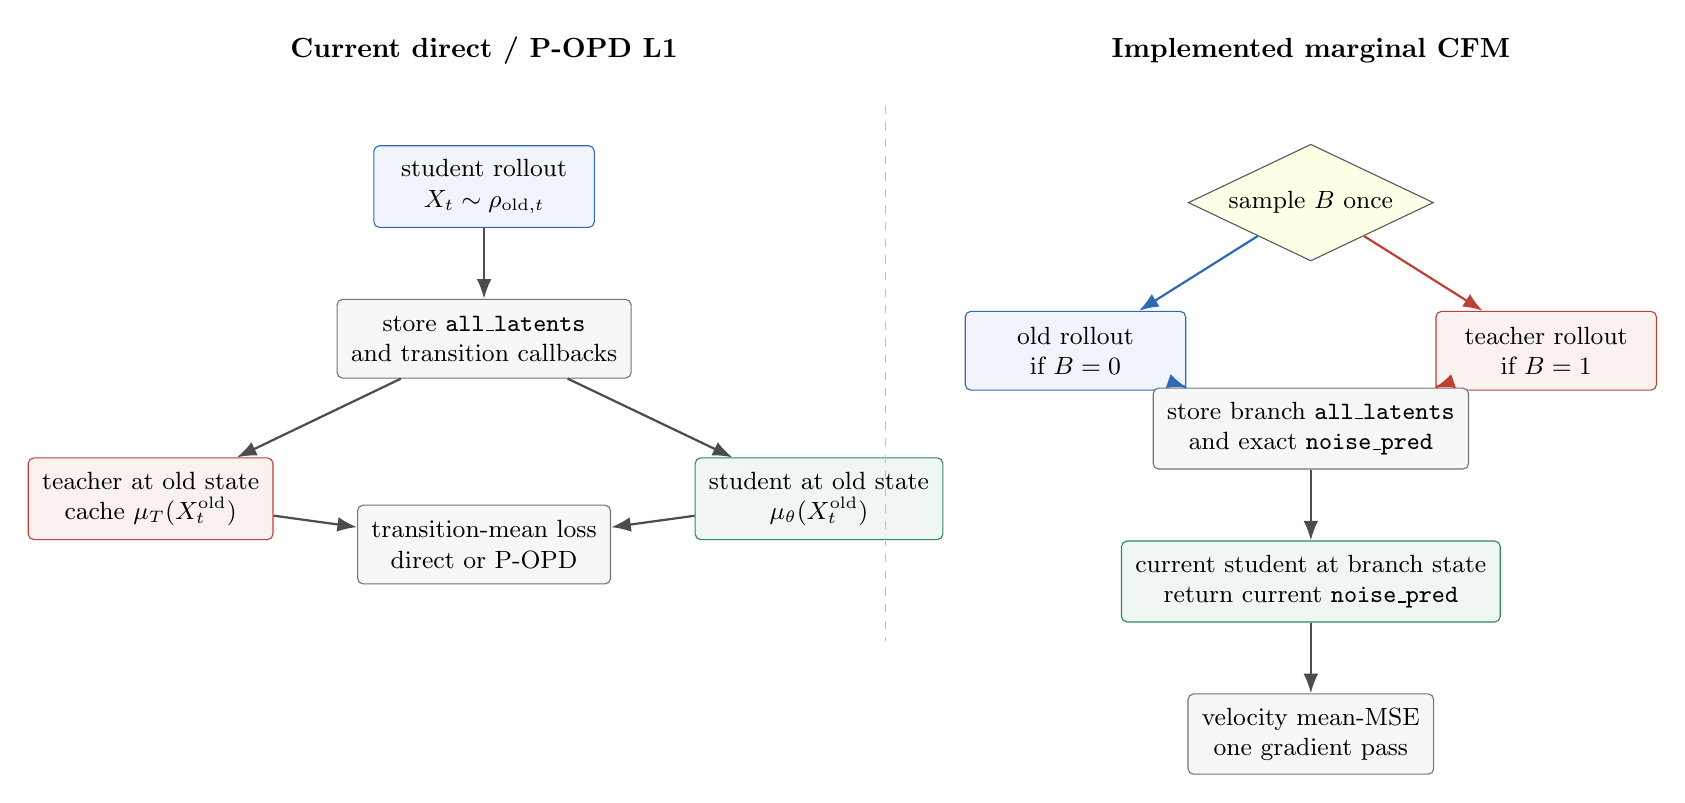
\begin{tikzpicture}[node distance=9mm and 17mm]
  % Current column
  \node[font=\bfseries] (ctitle) {Current direct / P-OPD L1};
  \node[oldbox,below=of ctitle] (croll) {student rollout\\$X_t\sim\rho_{\mathrm{old},t}$};
  \node[neutralbox,below=of croll] (cstore) {store \texttt{all\_latents}\\and transition callbacks};
  \node[teacherbox,below left=10mm and 8mm of cstore] (cpre) {teacher at old state\\cache $\mu_T(X_t^{\mathrm{old}})$};
  \node[studentbox,below right=10mm and 8mm of cstore] (cgrad) {student at old state\\$\mu_\theta(X_t^{\mathrm{old}})$};
  \node[neutralbox,below=16mm of cstore] (closs) {transition-mean loss\\direct or P-OPD};
  \draw[flowarrow] (croll) -- (cstore);
  \draw[flowarrow] (cstore) -- (cpre);
  \draw[flowarrow] (cstore) -- (cgrad);
  \draw[flowarrow] (cpre) -- (closs);
  \draw[flowarrow] (cgrad) -- (closs);

  % Divider
  \draw[dashed,black!25] (5.1,-0.7) -- (5.1,-7.5);

  % A4 column
  \begin{scope}[xshift=10.5cm]
    \node[font=\bfseries] (atitle) {Implemented marginal CFM};
    \node[decision,below=of atitle] (abranch) {sample $B$ once};
    \node[oldbox,below left=10mm and 8mm of abranch] (aold) {old rollout\\if $B=0$};
    \node[teacherbox,below right=10mm and 8mm of abranch] (ateacher) {teacher rollout\\if $B=1$};
    \node[neutralbox,below=16mm of abranch] (astore) {
      store branch \texttt{all\_latents}\\and exact \texttt{noise\_pred}
    };
    \node[studentbox,below=of astore] (astudent) {
      current student at branch state\\return current \texttt{noise\_pred}
    };
    \node[neutralbox,below=of astudent] (aloss) {velocity mean-MSE\\one gradient pass};
    \draw[flowarrow,draw=oldblue] (abranch) -- (aold);
    \draw[flowarrow,draw=teacherred] (abranch) -- (ateacher);
    \draw[flowarrow,draw=oldblue] (aold) -- (astore);
    \draw[flowarrow,draw=teacherred] (ateacher) -- (astore);
    \draw[flowarrow] (astore) -- (astudent);
    \draw[flowarrow] (astudent) -- (aloss);
  \end{scope}
\end{tikzpicture}
}
\caption{Direct/P-OPD XOPD queries the teacher on old states.  Implemented A4 routes each sample through
one source trajectory, captures that source's velocity, and removes the teacher pre-pass.}
\label{fig:code-pipeline}
\end{figure}

\subsection{One subtle conditioning issue}

Teacher rollout must use its dedicated prompt embeddings and text ids.  The returned sample,
however, stores whichever embeddings were active during that inference call.  Before
teacher-branch samples enter the student gradient pass, their ordinary student-conditioning
fields must be restored from the original dataloader rows:
\begin{equation}
\text{teacher trajectory state/target}
\quad+\quad
\text{student prompt conditioning for }v_\theta.
\label{eq:conditioning-separation}
\end{equation}
Failing to restore them would train the smaller student with teacher-encoder embeddings and would
no longer match normal student inference.

%% ============================================================
\section{Implemented same-VAE XOPD path}
\label{sec:implementation}
%% ============================================================

\begin{tcolorbox}[colback=green!5,colframe=green!50!black,title=Status]
\raggedright
A4 is implemented as \texttt{xopd\_target\_mode: marginal\_cfm}.
The production path is in \path{src/flow_factory/trainers/xopd/trainer.py} and
\path{src/flow_factory/trainers/xopd/common.py}.
Focused coverage is in \path{tests/test_marginal_cfm_trainer.py},
\path{tests/test_xopd_helpers.py}, and \path{tests/test_xopd_configs.py}.
\end{tcolorbox}

\subsection{Configuration}

Use a dedicated alpha rather than overloading \texttt{popd\_alpha}; the latter is a transition
mixture prior with different diagnostics and validity conditions.

\begin{lstlisting}[style=yaml,caption={Implemented same-VAE A4 configuration.}]
train:
  trainer_type: xopd
  xopd_target_mode: marginal_cfm
  marginal_cfm_alpha: 0.5

  # A4 always matches source velocity.
  xopd_dk_space: v
  normalize_d_k: false
  pathwise_coef: 1.0

  # Existing timestep selection and one-step-per-epoch geometry remain.
  num_xopd_steps: 4
  xopd_step_sampling: stratified

scheduler:
  dynamics_type: ODE
  noise_level: 0.0
\end{lstlisting}

The implemented field is a single static scalar.  It is read for every branch draw but is not
scheduled by epoch, optimizer step, or ODE time.  Section~\ref{sec:dynamic-alpha} is therefore
theory and experiment design, not a claim that dynamic alpha is already supported.  A future
outer-loop schedule must resolve one scalar $\alpha_k$ before branch sampling and keep it fixed
for the full trajectory.

The implementation enforces these fail-fast checks:
\begin{enumerate}[leftmargin=1.6em]
\item \texttt{dynamics\_type == "ODE"};
\item $0\le\texttt{marginal\_cfm\_alpha}\le1$ and finite;
\item same VAE / same latent state space; reject cross-VAE transport and pixel loss;
\item \texttt{xopd\_dk\_space == "v"} and \texttt{normalize\_d\_k == false};
\item teacher and student rollout grids, latent shapes, and selected steps agree;
\item every selected callback index is nonnegative and every target is finite.
\end{enumerate}

\paragraph{Implemented touch points.}
The mode is wired through the complete rollout/replay path:
\begin{enumerate}[leftmargin=1.6em]
\item the target-mode literal and dedicated A4 alpha live in XOPD training arguments;
\item the trainer derives \texttt{\_is\_marginal\_cfm} at initialization;
\item target-mode-specific validation preserves direct and P-OPD behavior;
\item A4 validation enforces the ODE, same-VAE, and \texttt{v}-space matrix;
\item both \texttt{sample()} and \texttt{optimize()} dispatch through A4-specific target handling;
\item canonical validation and matched smoke configs serialize the target fields;
\item the direct-XOPD validation-$D_k$ evaluator is skipped in A4 mode, because it
      queries the teacher on student states rather than evaluating held-out marginal CFM.
\end{enumerate}

\subsection{Step 1: draw one branch before rollout}

\begin{lstlisting}[style=python,caption={Implemented deterministic branch draw.}]
branches = draw_marginal_cfm_branches(
    batch_size,
    alpha=self.training_args.marginal_cfm_alpha,
    seed=self.training_args.seed,
    epoch=self.epoch,
    batch_index=batch_index,
)
\end{lstlisting}

Draw the labels before calling \texttt{inference}.  Split the dataloader batch into old and
teacher row subsets.  Each row runs exactly one ODE trajectory:
\begin{equation}
\text{expected rollout cost per sample}
=(1-\alpha)C_{\mathrm{old}}+\alpha C_T.
\label{eq:rollout-cost}
\end{equation}
Running a student trajectory for every row and an additional teacher trajectory for $B=1$ rows
would cost $C_{\mathrm{old}}+\alpha C_T$ and store unnecessary paths.

\begin{tcolorbox}[colback=red!4,colframe=red!45!black,title=Distributed call-order invariant]
For the first FSDP implementation, all ranks must draw the \emph{same branch pattern} and have the
same local batch geometry.  The seed above intentionally excludes rank.  Then every rank enters
the old and teacher transformer collectives in the same order with the same subset sizes.  Adding
rank to the seed can make one rank skip a teacher call while another enters it, which can
deadlock.  The cost is correlated branch labels across ranks; independent routing would require
an always-call/padded collective design.
\end{tcolorbox}

\subsection{Step 2: route the two subsets and capture the source velocity}

\texttt{\_slice\_marginal\_cfm\_batch\_rows} preserves row-aligned tensor/list fields and shared
objects, while \texttt{\_sample\_marginal\_cfm\_batch} handles empty subsets, restores original
row order before metadata stitching, and offloads the merged samples through the normal sample
lifecycle.  Nested I2I inputs and positive/negative prompt embeddings plus text ids are covered by
the same routing and restoration path.

\begin{lstlisting}[style=python,caption={Implemented A4 sampling structure, abbreviated.}]
def _sample_marginal_cfm_batch(
    self,
    batch: Dict[str, Any],
    batch_index: int,
    trajectory_indices: List[int],
) -> List[BaseSample]:
    batch_size = int(batch["prompt_embeds"].shape[0])
    branches = draw_marginal_cfm_branches(
        batch_size,
        alpha=self.training_args.marginal_cfm_alpha,
        seed=self.training_args.seed,
        epoch=self.epoch,
        batch_index=batch_index,
    )
    result: List[Optional[BaseSample]] = [None] * batch_size

    for use_teacher in (False, True):
        row_indices = torch.nonzero(
            branches == use_teacher, as_tuple=False
        ).flatten()
        if row_indices.numel() == 0:
            continue

        subset = self._slice_marginal_cfm_batch_rows(
            batch, row_indices, batch_size
        )
        infer_kwargs = {
            **self.training_args,
            **subset,
            "compute_log_prob": False,
            "trajectory_indices": trajectory_indices,
            "extra_call_back_kwargs": ["noise_pred"],
            "guidance_scale": (
                self.teacher_gs if use_teacher else self.student_gs
            ),
        }

        if use_teacher:
            self._route_marginal_cfm_teacher_conditioning(
                infer_kwargs, subset
            )
            infer_kwargs = filter_kwargs(
                self.adapter.inference, **infer_kwargs
            )
            with self.adapter.use_teacher_transformer():
                subset_samples = self.adapter.inference(**infer_kwargs)
            self._restore_marginal_cfm_student_conditioning(
                subset_samples, subset
            )
        else:
            infer_kwargs = filter_kwargs(
                self.adapter.inference, **infer_kwargs
            )
            subset_samples = self.adapter.inference(**infer_kwargs)

        expected_count = int(row_indices.numel())
        if len(subset_samples) != expected_count:
            raise RuntimeError(
                "marginal CFM subset rollout count mismatch: "
                f"use_teacher={use_teacher}, "
                f"expected={expected_count}, "
                f"received={len(subset_samples)}."
            )
        for original_row, sample in zip(
            row_indices.tolist(), subset_samples
        ):
            sample.extra_kwargs["marginal_cfm_branch"] = torch.tensor(
                use_teacher, dtype=torch.bool
            )
            result[original_row] = sample

    if any(sample is None for sample in result):
        missing = [i for i, sample in enumerate(result) if sample is None]
        raise RuntimeError(
            "marginal CFM rollout did not produce one sample per input row; "
            f"missing_rows={missing}, batch_size={batch_size}."
        )

    merged: List[BaseSample] = []
    for sample in result:
        if sample is None:
            raise RuntimeError(
                "marginal CFM internal merge invariant failed after "
                "the missing-row check."
            )
        merged.append(sample)
    stitch_batch_metadata(batch, merged)
    self._maybe_offload_samples_to_cpu(merged)
    return merged
\end{lstlisting}

\paragraph{Teacher conditioning helpers.}
The routing helper must fail if teacher-side positive conditioning is absent, and must also
require teacher-side negative conditioning whenever teacher CFG is active:
\begin{lstlisting}[style=python,caption={Implemented teacher-conditioning replacement rules, abbreviated.}]
def _route_marginal_cfm_teacher_conditioning(
    self,
    inference_kwargs: Dict[str, Any],
    subset: Dict[str, Any],
) -> None:
    required = ("teacher_prompt_embeds", "teacher_text_ids")
    missing = [key for key in required if subset.get(key) is None]
    if missing:
        raise ValueError(
            "marginal CFM teacher rollout requires teacher conditioning, "
            f"missing_keys={missing!r}."
        )

    device = self.accelerator.device
    inference_kwargs["prompt_embeds"] = subset[
        "teacher_prompt_embeds"
    ].to(device)
    inference_kwargs["text_ids"] = subset["teacher_text_ids"].to(device)
    inference_kwargs.pop("prompt_ids", None)

    negative_keys = (
        "teacher_negative_prompt_embeds",
        "teacher_negative_text_ids",
    )
    if self.teacher_gs > 1.0:
        missing_negative = [
            key for key in negative_keys if subset.get(key) is None
        ]
        if missing_negative:
            raise ValueError(
                "marginal CFM teacher CFG requires negative teacher "
                f"conditioning, missing_keys={missing_negative!r}, "
                f"teacher_guidance_scale={self.teacher_gs}."
            )
        inference_kwargs["negative_prompt_embeds"] = subset[
            "teacher_negative_prompt_embeds"
        ].to(device)
        inference_kwargs["negative_text_ids"] = subset[
            "teacher_negative_text_ids"
        ].to(device)
        inference_kwargs.pop("negative_prompt_ids", None)
    else:
        for key in (
            "negative_prompt_embeds",
            "negative_text_ids",
            "negative_prompt_ids",
        ):
            inference_kwargs.pop(key, None)
\end{lstlisting}

After inference, restore these student-side sample fields from the subset rows:
\[
\begin{gathered}
\texttt{prompt\_ids},\ \texttt{prompt\_embeds},\ \texttt{text\_ids},\\
\texttt{negative\_prompt\_ids},\
\texttt{negative\_prompt\_embeds},\
\texttt{negative\_text\_ids}.
\end{gathered}
\]
Keep the teacher-specific fields untouched for diagnostics.  Row slicing/restoration must also
preserve nested I2I conditions rather than assuming every value is a dense tensor.

Three details are correctness-critical:
\begin{enumerate}[leftmargin=1.6em]
\item \texttt{extra\_call\_back\_kwargs=["noise\_pred"]} is necessary.  Including
      \texttt{noise\_pred} in internal \texttt{return\_kwargs} alone does not make
      \texttt{CallbackCollector} store it.
\item Teacher samples keep teacher trajectory latents and callback targets, but their ordinary
      prompt fields are restored to the student conditioning.
\item The teacher context is no-grad and uses
      \texttt{adapter.use\_teacher\_transformer()}, which already swaps away from the wrapped
      student and disables the autocast cache for the scope.
\end{enumerate}

\subsection{Step 3: align the state and callback target}

After \texttt{BaseSample.stack}, expected shapes are
\begin{center}
\begin{tabular}{@{}lll@{}}
\toprule
field & shape & meaning\\
\midrule
\texttt{all\_latents} & $(B,T_x,\ldots)$ & selected state positions\\
\texttt{latent\_index\_map} & $(T+1,)$ & full position $\to$ compact state index\\
\texttt{noise\_pred} & $(B,T_v,\ldots)$ & selected source velocities\\
\texttt{callback\_index\_map} & $(B,T)$ before normalization & full step $\to$ compact callback index\\
\texttt{marginal\_cfm\_branch} & $(B,)$ & diagnostic source label\\
\bottomrule
\end{tabular}
\end{center}

\begin{lstlisting}[style=python,caption={Correct state/velocity alignment after map normalization.}]
latent_compact_index = int(latent_index_map[timestep_index])
callback_compact_index = int(callback_index_map[timestep_index])

if latent_compact_index < 0 or callback_compact_index < 0:
    raise RuntimeError(
        "marginal CFM selected an uncollected trajectory step: "
        f"timestep_index={timestep_index}, "
        f"latent_compact_index={latent_compact_index}, "
        f"callback_compact_index={callback_compact_index}."
    )

latents = batch["all_latents"][:, latent_compact_index]
velocity_target = batch["noise_pred"][
    :, callback_compact_index
].detach()
\end{lstlisting}

Do not index \texttt{noise\_pred} with \texttt{latent\_index\_map}: callbacks index transitions,
whereas latent storage indexes positions.

\subsection{Step 4: keep the existing optimizer shell}

The safest implementation does \emph{not} create a second copy of the optimizer loop.  Extend the
existing \texttt{\_optimize\_train\_pass} pathwise-loss dispatch, while preserving its exact
ordering:
\[
\begin{aligned}
\text{accumulate}
&\to
\text{student forward}
\to
\text{pathwise + auxiliary + KL losses}\\
&\to
\text{backward}
\to
\text{clip / step / zero}.
\end{aligned}
\]
The student return-key helper must always request \texttt{noise\_pred} in A4 mode.

\begin{lstlisting}[style=python,caption={Implemented A4 branch inside the existing optimizer shell, abbreviated.}]
with self.accelerator.accumulate(*self.adapter.trainable_components):
    # Build batched t, t_next, latents, and next_latents exactly as
    # the current _optimize_train_pass does.
    forward_kwargs = self._build_forward_kwargs(
        batch=batch,
        t=t,
        t_next=t_next,
        latents=latents,
        next_latents=next_latents,
        compute_log_prob=False,
        return_kwargs=self._student_return_kwargs_for_train(),
        guidance_scale=self.student_gs,
    )
    student_out = self.adapter.forward(**forward_kwargs)

    if self._is_marginal_cfm:
        callback_index = resolve_marginal_cfm_callback_index(
            callback_index_map,
            timestep_index=timestep_index,
            callback_count=int(batch["noise_pred"].shape[1]),
        )
        target_noise_pred = batch["noise_pred"][
            :, callback_index
        ].detach()
        if student_out.noise_pred is None:
            raise RuntimeError(
                "marginal CFM requires current student `noise_pred`; "
                f"got None at timestep_index={timestep_index}."
            )
        d_k_grad = compute_marginal_cfm_velocity_loss(
            student_out.noise_pred,
            target_noise_pred,
        )
        diagnostics = compute_marginal_cfm_diagnostics(
            student_noise_pred=student_out.noise_pred,
            target_noise_pred=target_noise_pred,
            teacher_branch_mask=batch["marginal_cfm_branch"],
        )
        self._append_marginal_cfm_diagnostics(
            loss_info,
            diagnostics,
            batch["marginal_cfm_branch"],
        )
    elif self._is_popd:
        # Existing P-OPD branch remains unchanged.
        d_k_grad = compute_popd_pathwise_term(...)
    else:
        # Existing direct / pixel branches remain unchanged.
        d_k_grad = compute_direct_pathwise_term(...)

    pathwise_loss = d_k_grad.mean()
    loss = self.pathwise_coef * pathwise_loss

    # The existing inline MoE/MoF auxiliary-loss blocks add to loss here.
    if self.enable_kl_loss:
        kl_div, kl_loss = self._compute_kl_anchor(
            student_out, forward_kwargs
        )
        loss = loss + kl_loss

    # Backward occurs only after every differentiable term is added.
    self.accelerator.backward(loss)
    if self.accelerator.sync_gradients:
        grad_norm = self._clip_grad_norm_ep_aware(...)
        self.optimizer.step()
        self.optimizer.zero_grad()
        # Keep the existing reduce/log/step bookkeeping.
\end{lstlisting}

The P-OPD/direct branches and inline auxiliary blocks are abbreviated in the listing; the A4
helper names are the production symbols.  The number of backward calls remains
\[
\texttt{num\_batches\_per\_epoch}
\times
\texttt{num\_train\_timesteps},
\]
so the existing one-optimizer-step-per-epoch GAS invariant remains valid.

\subsection{Dispatch changes}

The high-level branch in \texttt{optimize()} skips only target precomputation; every mode
then enters the shared optimizer shell:
\begin{lstlisting}[style=python,caption={Implemented target-mode dispatch, abbreviated.}]
if self._is_marginal_cfm:
    mu_teacher_list = None
    popd_cache_list = None
    callback_index_map = normalize_callback_index_map(
        batch["callback_index_map"]
    )
else:
    mu_teacher_list = self._precompute_teacher_means(...)
    popd_cache_list = (
        self._precompute_popd_step_caches(...)
        if self._is_popd else None
    )
    callback_index_map = None

loss_info = self._optimize_train_pass(
    ...,
    mu_teacher_list=mu_teacher_list,
    popd_cache_list=popd_cache_list,
    callback_index_map=callback_index_map,
)
\end{lstlisting}

A4 must not call \texttt{\_precompute\_teacher\_means}: the exact branch target has already been
captured during the source rollout.  The shared optimizer signature must make
\texttt{mu\_teacher\_list} and \texttt{popd\_cache\_list} optional, and every access to them must
remain inside the direct/P-OPD branches.  The student return-key helper must add
\texttt{noise\_pred} whenever \texttt{self.\_is\_marginal\_cfm} is true.

\subsection{Compute and memory}

For $B$ samples and $K$ trained steps:
\begin{center}
\begin{tabular}{@{}
  >{\raggedright\arraybackslash}p{0.18\textwidth}
  >{\raggedright\arraybackslash}p{0.29\textwidth}
  >{\raggedright\arraybackslash}p{0.25\textwidth}
  >{\raggedright\arraybackslash}p{0.18\textwidth}
@{}}
\toprule
design & rollout forwards & optimize forwards & trajectory storage\\
\midrule
direct XOPD
& $B$ student trajectories
& $BK$ teacher + $BK$ student
& states\\
implemented A4
& $(1-\alpha)B$ old + $\alpha B$ teacher trajectories
& $BK$ student
& states + $T_v$ velocities\\
dual-rollout A4
& $B$ old + $\alpha B$ teacher trajectories
& $BK$ student
& extra teacher states\\
\bottomrule
\end{tabular}
\end{center}

The implemented design removes the teacher pre-pass but stores one velocity tensor for every callback
step.  Do not assume $T_v=K$: the current trajectory-index expansion can collect neighboring
positions and make $T_v$ approach $2K$.  Either introduce a separate callback-step selector or
measure and report the actual compact callback length.  With all steps stored, callback storage
is roughly another trajectory-sized tensor.

%% ============================================================
\section{Validation, diagnostics, and implementation checklist}
\label{sec:validation}
%% ============================================================

\subsection{Unit tests}

The focused implementation tests cover:
\begin{enumerate}[leftmargin=1.6em]
\item \textbf{Branch frequency}: a large deterministic draw approaches $\alpha$ and is repeatable
      for the same seed/epoch/batch index.
\item \textbf{Boundary cases}: $\alpha=0$ produces only old branches; $\alpha=1$ produces only
      teacher branches.
\item \textbf{Branch lifetime}: one label is attached to the entire sample and never redrawn per
      timestep.
\item \textbf{Index alignment}: real \texttt{Flux2KleinSample} objects passed through
      \texttt{BaseSample.stack} produce a $(B,T)$ callback map, normalize correctly, retrieve the
      intended state/target, and raise on $-1$.
\item \textbf{Gradient ownership}: target callbacks and teacher parameters have no gradient;
      current student parameters do.
\item \textbf{Source correctness}: teacher branch states come from teacher inference, not teacher
      forwards on old states.
\item \textbf{Conditioning restoration}: positive and negative prompt embeddings plus text ids are
      restored to student values after teacher rollout.
\item \textbf{Storage lifecycle}: branch labels, callback tensors, and maps survive CPU offload,
      device reload, shuffling, and stacking.
\item \textbf{Optimizer integration}: MoE/MoF auxiliaries and the optional KL anchor contribute
      gradients before backward; GAS still yields one optimizer step per epoch.
\item \textbf{Distributed call-order protocol}: the rank-independent branch draw and fixed
      old-then-teacher subset order are deterministic, including empty subsets.
\item \textbf{Shape/finite guards}: mismatched shape, NaN, or Inf raises an informative error.
\end{enumerate}

\begin{lstlisting}[style=python,caption={Representative implemented helper-level assertions.}]
def test_marginal_cfm_loss_only_gradients_student():
    velocity_student = torch.tensor([[1.0, 2.0]], requires_grad=True)
    velocity_target = torch.tensor([[0.0, 4.0]], requires_grad=False)

    loss = (velocity_student - velocity_target).square().mean()
    loss.backward()

    assert velocity_student.grad is not None
    assert velocity_target.grad is None


def test_callback_map_shape_after_real_sample_stack():
    map_per_sample = torch.tensor([-1, -1, 0, -1])
    samples = [
        Flux2KleinSample(
            extra_kwargs={
                "callback_index_map": map_per_sample,
                "marginal_cfm_branch": torch.tensor(False),
            },
        ),
        Flux2KleinSample(
            extra_kwargs={
                "callback_index_map": map_per_sample.clone(),
                "marginal_cfm_branch": torch.tensor(True),
            },
        ),
    ]

    batch = BaseSample.stack(samples)
    assert batch["callback_index_map"].shape == (2, 4)
    callback_map = normalize_callback_index_map(
        batch["callback_index_map"]
    )
    assert torch.equal(callback_map, map_per_sample)
    assert batch["marginal_cfm_branch"].shape == (2,)
\end{lstlisting}

\subsection{GPU smoke tests}

The checked-in pair holds the prompt source, model, timestep schedule, batch/GAS geometry, and
optimizer settings fixed.  Only the target behavior changes:
\begin{lstlisting}[style=yaml,caption={Matched eight-GPU smoke commands.}]
ff-train xopd_configs/ode_pathwise/_TEST_9b_4b_marginal_cfm_smoke.yaml
ff-train xopd_configs/ode_pathwise/_TEST_9b_4b_direct_ctrl_marginal_cfm_smoke.yaml
\end{lstlisting}
The A4 config uses $\alpha=0.5$; $\alpha=0$ and $\alpha=1$ routing boundaries are covered by CPU
unit tests.  These commands are documented but were \textbf{NOT RUN locally} and are
\textbf{not evidence of passing distributed validation}.  The real smoke requires an eight-GPU
host.
Check:
\begin{itemize}[leftmargin=1.5em]
\item exactly one optimizer step per epoch;
\item no call to \texttt{\_precompute\_teacher\_means} in A4 mode;
\item finite loss and gradient norm;
\item callback/state maps align at every selected step;
\item teacher swap scope restores the wrapped student component;
\item MoE/MoF and KL-anchor losses are included before backward;
\item the legacy direct validation-$D_k$ path is disabled or explicitly relabeled in A4 mode;
\item eval generation still uses the ordinary student ODE.
\end{itemize}

\subsection{Diagnostics}

The shared \texttt{reduce\_loss\_info} reducer preserves scalar keys and expands every
per-sample vector into \texttt{\_min}, \texttt{\_max}, \texttt{\_mean}, and \texttt{\_std}
series.  The overall objective and matching term therefore remain the scalar
\path{train/loss} and \path{train/d_k} keys; there is no
\path{train/marginal_cfm/loss}.  In the table, A4 base names are under
\path{train/marginal_cfm/}; ``four stats'' means all four suffixes above.
\begin{center}
\begin{tabular}{@{}
  >{\raggedright\arraybackslash}p{0.42\textwidth}
  >{\raggedright\arraybackslash}p{0.50\textwidth}
@{}}
\toprule
metric & purpose\\
\midrule
\path{train/loss}, \path{train/d_k}
& scalar overall objective and CFM matching term\\
\path{train/loss/\{ti\}}, \path{train/d_k/\{ti\}}
& scalar per-timestep objective and matching term\\
\texttt{callback\_count}
& measure actual compact callback storage\\
\texttt{teacher\_branch\_fraction} (four stats)
& verify Bernoulli routing and distributed aggregation\\
\texttt{scheduled alpha} and cumulative $A_{\mathrm{eff}}$
& required if an outer-loop alpha schedule is implemented\\
\texttt{loss\_old}, \texttt{loss\_teacher} (four stats)
& branch-conditioned fitting difficulty; absent for an empty branch\\
\texttt{target\_velocity\_rms} (four stats)
& resolution-stable target scale\\
\texttt{target\_velocity\_l2} (four stats)
& full event scale\\
\texttt{student\_target\_gap\_rms} (four stats)
& direct CFM fitting error\\
\path{train/grad_norm}
& distinguish small CFM error from optimizer clipping\\
\bottomrule
\end{tabular}
\end{center}

Do \emph{not} log a transition \texttt{gamma}: A4 never computes one.  A density-responsibility
estimate would be an optional research diagnostic, not part of the training algorithm.

\subsection{Implementation checklist}

\begin{tcolorbox}[colback=green!5,colframe=green!50!black,title=Minimum correct same-VAE A4]
\begin{enumerate}[leftmargin=1.5em]
\item[$\checkmark$] ODE-only, shared latent space, shared timestep grid.
\item[$\checkmark$] Draw one branch label per full trajectory before rollout.
\item[$\checkmark$] Run only the selected old or teacher trajectory for each row.
\item[$\checkmark$] Capture the selected source's CFG-combined \texttt{noise\_pred}.
\item[$\checkmark$] Restore student conditioning fields on teacher-trajectory samples.
\item[$\checkmark$] Align states with \texttt{latent\_index\_map} and targets with
      \texttt{callback\_index\_map}.
\item[$\checkmark$] Detach target velocities; backpropagate only through the current student.
\item[$\checkmark$] Skip the existing teacher-on-old-state pre-pass.
\item[$\checkmark$] Preserve accumulation, auxiliary losses, KL anchor, and optimizer boundaries.
\item[$\checkmark$] Preserve rank-synchronous old/teacher collective call order.
\item[$\checkmark$] Skip direct-XOPD validation-$D_k$ in A4 mode.
\item[$\checkmark$] Log branch fraction, per-branch losses, callback count, RMS/L2 scales, and
      gradient norm.
\end{enumerate}
\end{tcolorbox}

\subsection{Final mental model}

\begin{equation}
\boxed{
\begin{gathered}
\text{sample source branch}
\;\Longrightarrow\;
\text{sample source trajectory}
\;\Longrightarrow\;
\text{regress source velocity}\\[0.3em]
\text{CFM conditional averaging}
\;\Longrightarrow\;
u_t(x)
\;\Longrightarrow\;
q_t=(1-\alpha)\rho_{\mathrm{old},t}+\alpha\rho_{T,t}.
\end{gathered}
}
\label{eq:mental-model}
\end{equation}

The key is not to calculate the marginal responsibility.  The key is to sample the joint
distribution whose conditional mean \emph{is} the responsible mixture velocity.

\begin{thebibliography}{9}

\bibitem{flowmatching}
Yaron Lipman, Ricky T. Q. Chen, Heli Ben-Hamu, Maximilian Nickel, and Matt Le.
\newblock Flow Matching for Generative Modeling.
\newblock \emph{International Conference on Learning Representations}, 2023.
\newblock \url{https://arxiv.org/abs/2210.02747}.

\bibitem{diffusionopd}
Quanhao Li, Junqiu Yu, Kaixun Jiang, et al.
\newblock DiffusionOPD: A Unified Perspective of On-Policy Distillation in Diffusion Models.
\newblock 2026.
\newblock \url{https://arxiv.org/abs/2605.15055}.

\bibitem{topd}
Zhengpeng Xie, Li Lyna Zhang, Zeke Xie, and Mao Yang.
\newblock Trust Region Policy Distillation.
\newblock 2026.
\newblock \url{https://arxiv.org/abs/2607.04751}.

\end{thebibliography}

\end{document}
